\documentclass[11pt]{article} \usepackage{fullpage} \usepackage{graphicx} \usepackage{epstopdf} \usepackage{color} \usepackage{psfrag} \usepackage{pdfsync}\usepackage{indentfirst}\usepackage{subfigure}\usepackage{float}\usepackage[section]{placeins}
\usepackage{enumerate}
\usepackage{multirow}
\usepackage{amsfonts, fullpage, graphics} 
\usepackage{algorithm,algorithmic}
\usepackage{amsmath,amssymb,amsthm,bm,hyperref}
\usepackage{dsfont}
\usepackage[parfill]{parskip}
\usepackage[margin=1in]{geometry}
\newcommand{\Lagr}{\mathcal{L}}
\newcommand{\norm}[1]{\left\lVert#1\right\rVert}
\newcommand{\floor}[1]{\lfloor #1 \rfloor}
\newcommand{\todo}[1]{}
\renewcommand{\todo}[1]{{\color{red} TODO: {#1}}}
\newcommand\independent{\protect\mathpalette{\protect\independenT}{\perp}}
\newcommand{\obar}[1]{\mkern 1.5mu\overline{\mkern-1.5mu#1\mkern-1.5mu}\mkern 1.5mu}
\def\independenT#1#2{\mathrel{\rlap{$#1#2$}\mkern2mu{#1#2}}}
\newcommand{\rpm}{\sbox0{$1$}\sbox2{$\scriptstyle\pm$}
  \raise\dimexpr(\ht0-\ht2)/2\relax\box2 }
\usepackage{xspace}
\newcommand{\latex}{\LaTeX\xspace}
\setlength{\parindent}{2em}

\usepackage{listings}
\usepackage{color} %red, green, blue, yellow, cyan, magenta, black, white
\definecolor{mygreen}{RGB}{28,172,0} % color values Red, Green, Blue
\definecolor{mylilas}{RGB}{170,55,241}
\DeclareMathOperator{\E}{\mathbb{E}}
\DeclareMathOperator*{\argmax}{arg\,max}
\DeclareMathOperator*{\argmin}{arg\,min}

\begin{document}

{\parindent 0pt \begin{tabular}[t]{l} 16-720 Computer Vision \\ Spring 2020 \end{tabular}}%  \hfill XX/XX/14 \vskip 0.2in }
\parindent 0pt \parskip 8pt
\begin{center} \large\bf Homework 1 \end{center}
\begin{center} \large\bf Zongwen Mu, Andrew ID: zongwenm \end{center}
\bigskip


\section{Homographies}

\setcounter{subsection}{0}
\subsection{Homography}

\setlength{\parindent}{2em}  In this case, there exists matrices $P_1$, $P_2$ for two camera planes and plane $\boldsymbol{\Pi}$. The $P$ matrix could be written as $\left[ \begin{smallmatrix} A & b  \end{smallmatrix} \right]$, where $A$ has dimension $3*3$ and $b$ has dimension $1*1$. Since each $P$ is a projection matrix for one camera, the $det\left(A\right)$ for each projection matrix is not zero.

Therefore, there exists inverse matrix for $P$ to get a point's position in plane $\boldsymbol{\Pi}$. Thus, matrix $H$ for transition between plane $1$ and $2$ could be acquired by multiply one $P^{-1}$ with the other $P$.

\subsection{Correspondences}

\paragraph{1. How many degrees of freedom does h have?}~{}

Since there exists $\boldsymbol{H}$ such that:
\begin{equation}
	x_1^i \equiv Hx_2^i
\end{equation}

Therefore, we have:
\begin{equation}
	\begin{bmatrix}
	x_1 \\ y_1 \\ 1
	\end{bmatrix} = 
	\begin{bmatrix}
	h_{11} & h_{12} & h_{13} \\
	h_{21} & h_{22} & h_{23} \\
	h_{31} & h_{32} & h_{33}
	\end{bmatrix}
	\begin{bmatrix}
	x_2 \\ y_2 \\ 1
	\end{bmatrix}
\end{equation}

Rewrite $\bold{h}$ as:
\begin{equation}
	h = 
	\begin{bmatrix}
		h_{11} \\ h_{12} \\ h_{13} \\ h_{21} \\ h_{22} \\ h_{23} \\ h_{31} \\ h_{32} \\ h_{33}
	\end{bmatrix}
\end{equation}

There are 9 variables in $\boldsymbol{h}$, but we could normalize it by $h_{33}$, $\boldsymbol{h}$ will have 8 degrees of freedom.

\paragraph{2. How many point pairs are required to solve $h$?}~{}

$4$ point pairs are required.

\paragraph{3. Derive $A_i$}~{}

In part $1$, we acquired equations:
\begin{align}
	x_1 = h_{11}x_2 + h_{12}y_2 + h_{13} \\
	y_1 = h_{21}x_2 + h_{22}y_2 + h_{23} \\
	1 = h_{31}x_2 + h_{32}y_2 + h_{33}
\end{align}

Since $\bold{A_ih = 0}$, we could derive $\bold{A_i}$ as:
\begin{equation}
	A_i = 
	\begin{bmatrix}
		-x_2 & -y_2 & -1 & 0 & 0 & 0 & x_1x_2 & x_1y_2 & x_1 \\
		0 & 0 & 0 & -x_2 & -y_2 & -1 & y_1x_2 & y_1y_2 & y_1
	\end{bmatrix}
\end{equation}

\paragraph{4.}~{}

This could be solved in the least squares fashion, by finding the eigenvector of $\bold{A}$, corresponding to the smallest eigenvalue of $\bold{A}$.

Taking the SVD of $\bold{A}$:
\begin{equation}
	h = argmin\left(\left(h^{T}V\right)\Sigma^{2}\left(V^{T}h\right)\right)
\end{equation}

Therefore, $\bold{A}$ should be full rank, and $\bold{h}$ is the last column of $\bold{V}$.

\subsection{Homography Under Rotation}

Since there's no translation between world frame and two cameras, and there's no rotation for the first camera, we could find a inverse projection matrix for camera $1$, $M_1^{-1} = \left[ \begin{smallmatrix} I & 0  \end{smallmatrix} \right]^{T}K_1^{-1}$, and we could acquire $\bold{H}$ by $\boldsymbol{H} = M_1^{-1}K_2\left[ \begin{smallmatrix} R & 0  \end{smallmatrix} \right]$. Therefore, there exists a homography $\bold{H}$ between $\bold{x_1}$ and $\bold{x_2}$.

\subsection{Understanding Homographies Under Rotation}

Since $\bold{K}$ is constant, so the matrix $\bold{H^2}$ is corresponding to $\bold{R^2}$. For instance, if the camera is rotating around $\bold{z}$ axis:
\begin{align}
	\bold{R} = 
	\begin{bmatrix}
		\cos{\theta} & -\sin{\theta} & 0 \\
		\sin{\theta} & \cos{\theta} & 0 \\
		0 & 0 & 1
	\end{bmatrix} \\
	\bold{R^2} = 
	\begin{bmatrix}
		\cos{2\theta} & -\sin{2\theta} & 0 \\
		\sin{2\theta} & \cos{2\theta} & 0 \\
		0 & 0 & 1
	\end{bmatrix}
\end{align}

Therefore, $\bold{H^2}$ is corresponding to $2\theta$.

\subsection{Limitations of the Planar Homography}

The motion of camera may not be a pure rotation around its center or the points are not on a plane, thus planar homography is insufficient.

\subsection{Behavior of Lines Under Perspective Projections}

Point in world frame $\left[ \begin{smallmatrix} x & y & z \end{smallmatrix} \right]^{T}$ to point in projection $\left[ \begin{smallmatrix} x^\prime & y^\prime \end{smallmatrix} \right]^{T}$. Since for a line function in $3D$: 
\begin{equation}
	l\begin{bmatrix}
		x \\ y \\ z
	\end{bmatrix} = 0
\end{equation}

In 2d coordinate, we have:
\begin{equation}
	l\begin{bmatrix}
		\frac{x}{z} \\ \frac{y}{z} \\ 1
	\end{bmatrix} = 0
\end{equation}

Thus let $\frac{x}{z} = x^\prime$ and $\frac{y}{z} = y^\prime$, we have:
\begin{equation}
	l\begin{bmatrix}
		x^\prime \\ y^\prime \\ 1
	\end{bmatrix} = 0
\end{equation}

Therefore, the projection $\bold{P}$ preserve lines.

\section{Computing Planar Homographies}
\setcounter{subsection}{0}
\subsection{Feature Detection and Matching}

\setcounter{subsubsection}{0}
\subsubsection{FAST Detector}

FAST detector works by selecting pixel rather than using sliding window, and FAST detector would compare those pixels around selected pixel, and if there is enough pixels brighter or darker than selected pixel, this pixel is considered as a corner. Compared with Harris detector, FAST do not need to calculate $\lambda$ for whole sliding window, which would save great energy and time in computation.

\subsubsection{BRIEF Descriptor}

BRIEF would create a patch around selected point and implement Gaussian Filter to this region. Then it will randomly select $\bold{N}$ point pairs and compare each pair to acquire a binary code in length $\bold{N}$ as descriptor of this patch.

\subsubsection{Matching Methods}

When BRIEF descriptor acquired binary codes for two interest points, Hamming distance is calculating the XOR between two descriptors. Hamming distance benefits since it would be much easier for CPU to perform XOR and bit count operations.

\subsubsection{Feature Matching}

Result for default parameters is shown below:
\begin{figure}[H]
\centering
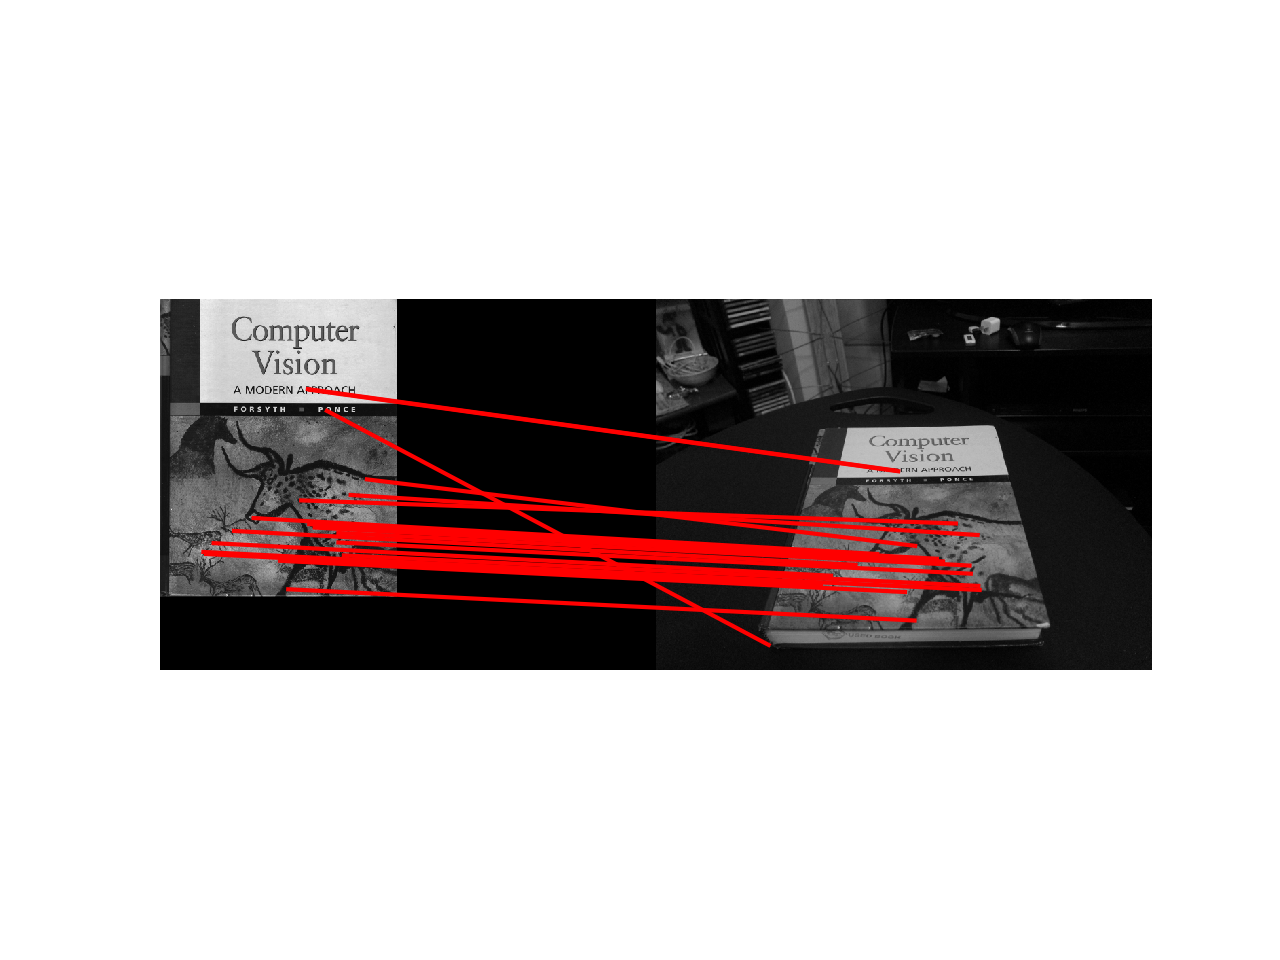
\includegraphics[width=0.5\textwidth]{results/q2_1_4_de.png}
\caption{resulting picture}
\end{figure}


\subsubsection{Feature Matching Parameter Tuning}
Firstly, I used fixed $sigma = 0.15$ and tuning $ratio$, the results are shown below:
\begin{figure}[H]
\centering
\subfigure[sigma=0.15 ratio=0.3]{
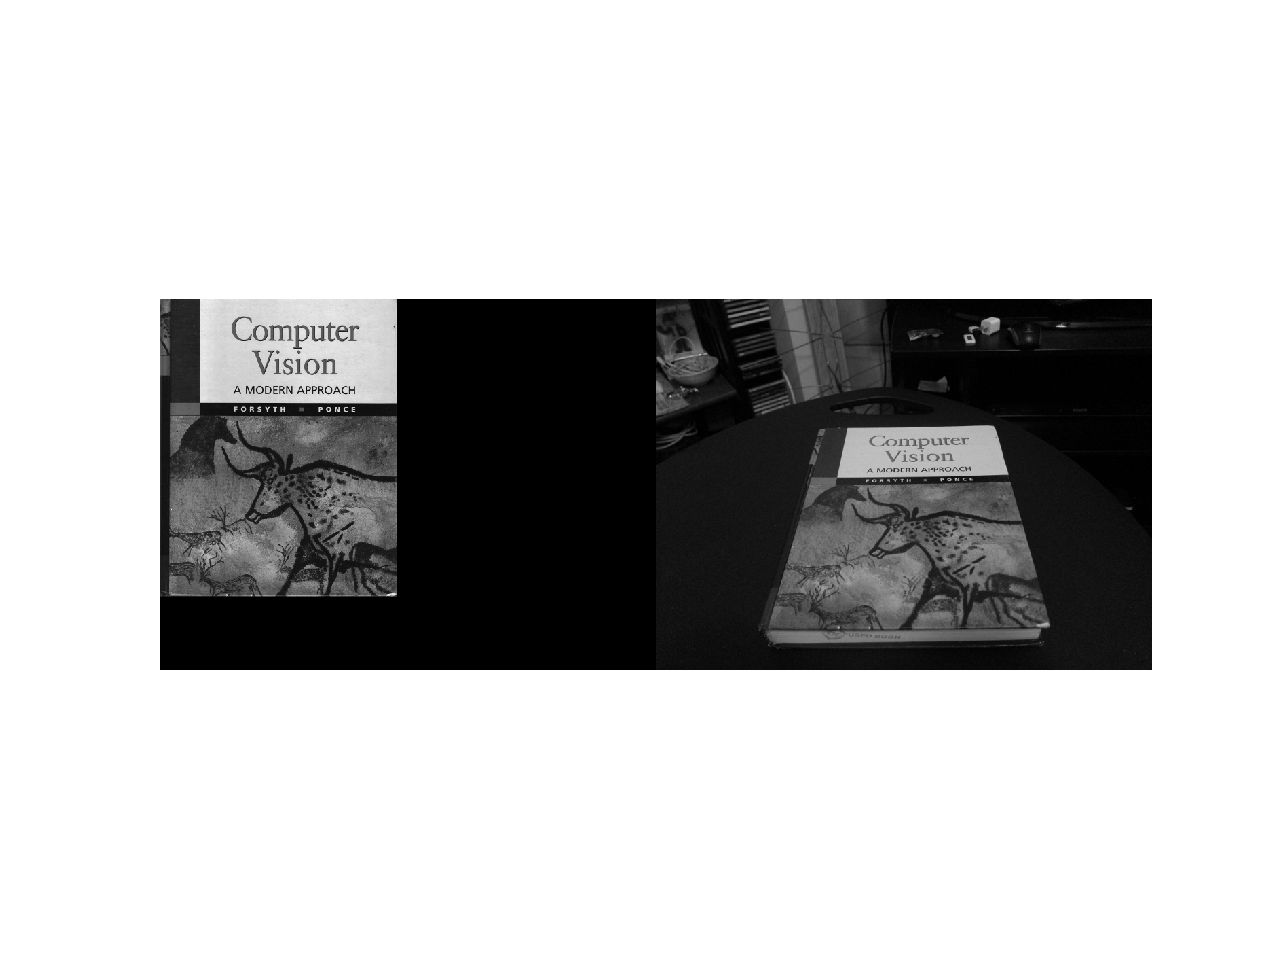
\includegraphics[width=0.4\textwidth]{results/q2_1_4_15_3.png}}
\subfigure[sigma=0.15 ratio=0.5]{
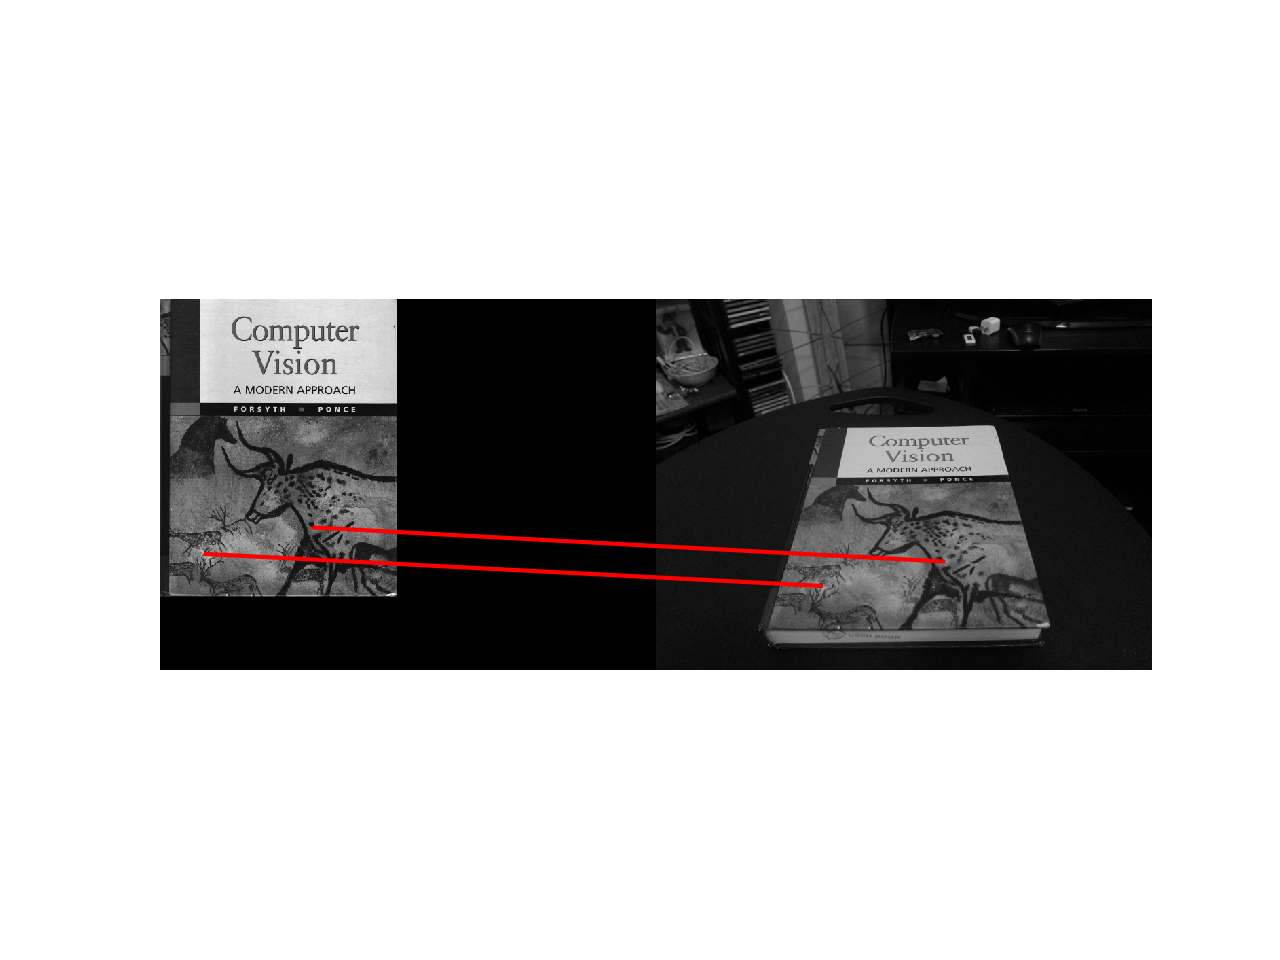
\includegraphics[width=0.4\textwidth]{results/q2_1_4_15_5.png}}
\subfigure[sigma=0.15 ratio=0.7]{
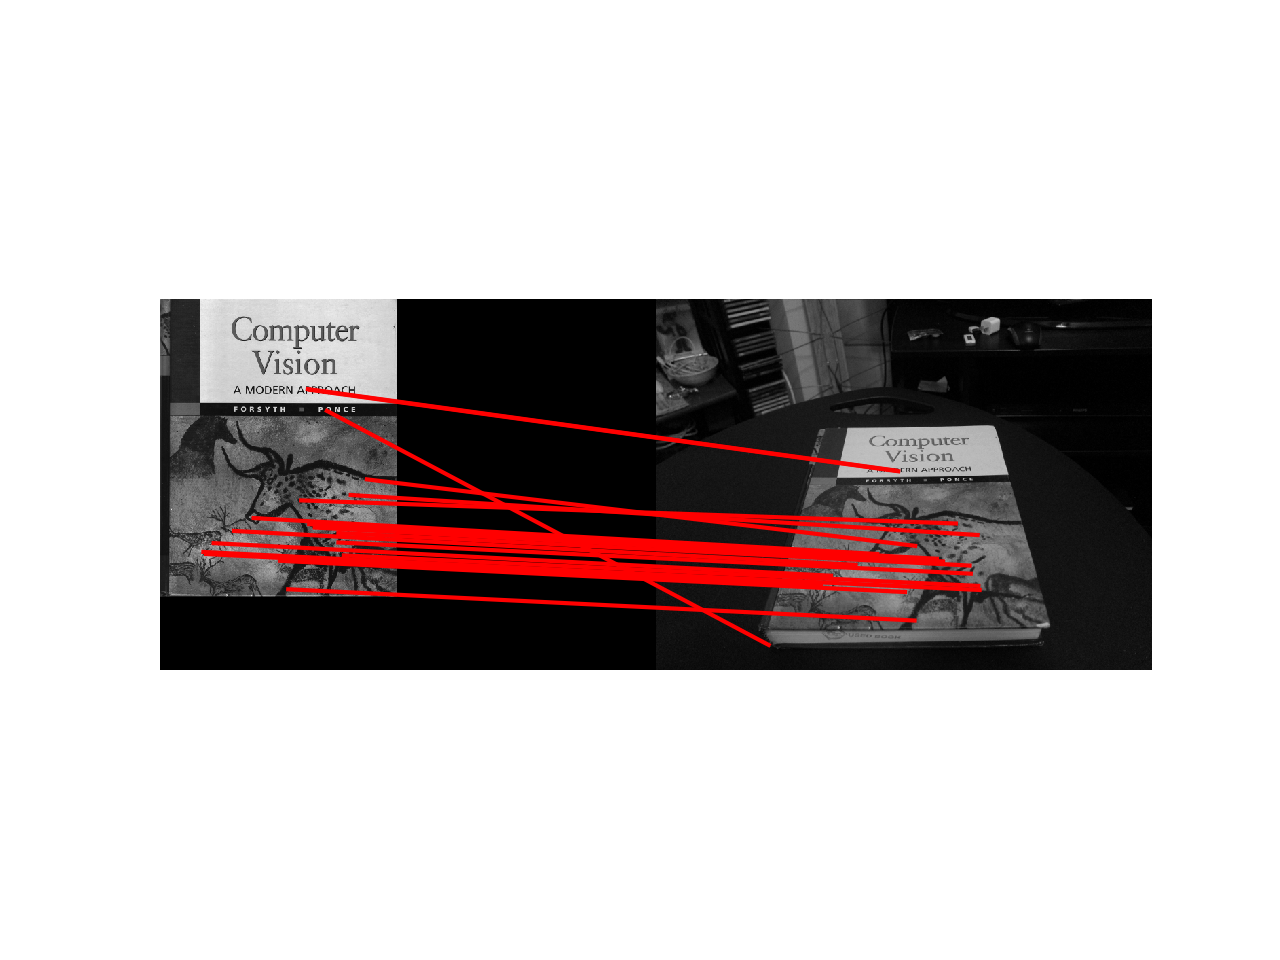
\includegraphics[width=0.4\textwidth]{results/q2_1_4_de.png}}
\subfigure[sigma=0.15 ratio=0.9]{
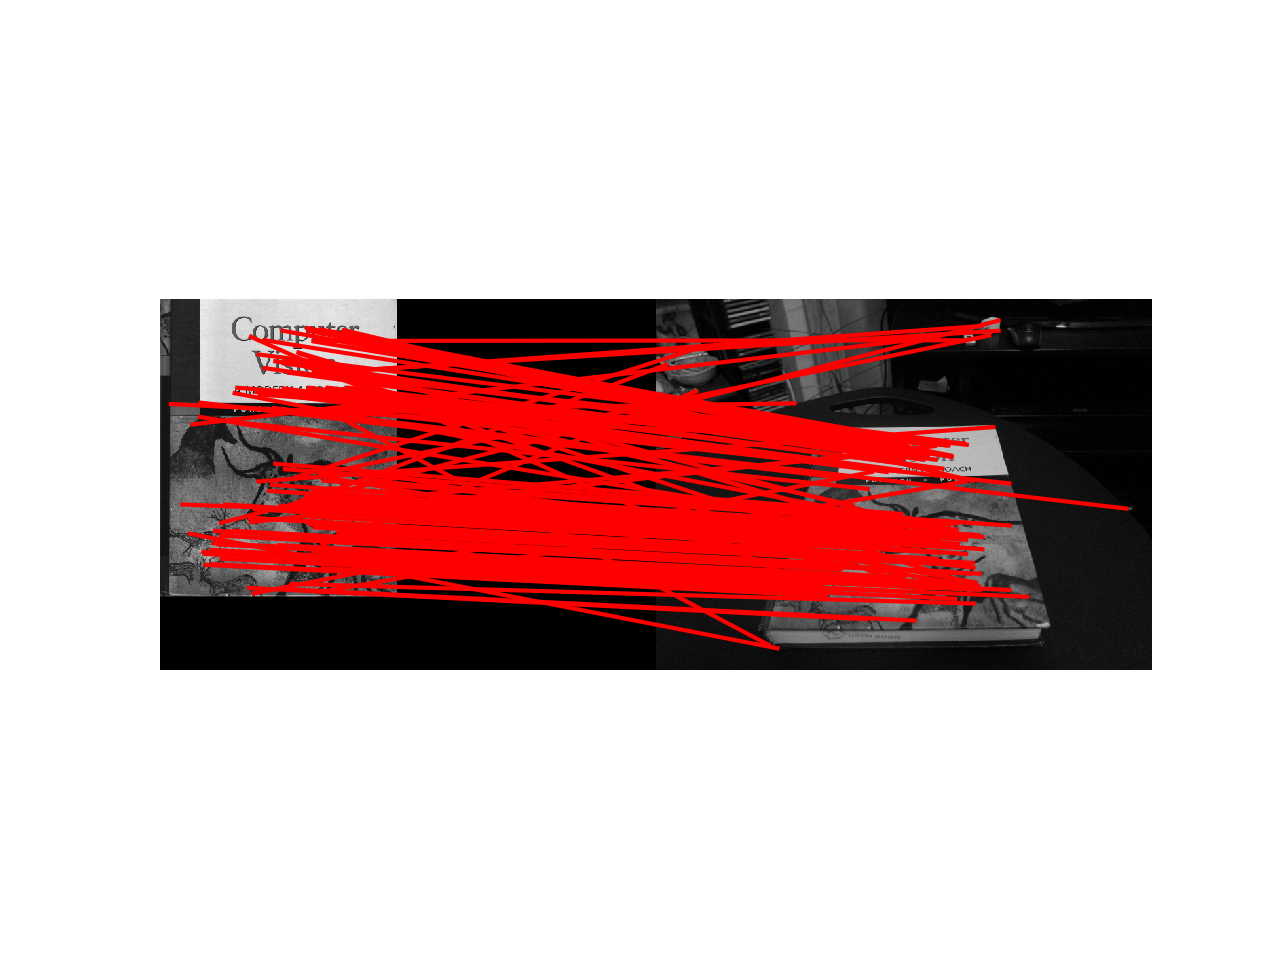
\includegraphics[width=0.4\textwidth]{results/q2_1_4_15_9.png}}
\end{figure}

Then using fixed $ration = 0.7$, tuning sigma:
\begin{figure}[H]
\centering
\subfigure[sigma=0.05 ratio=0.7]{
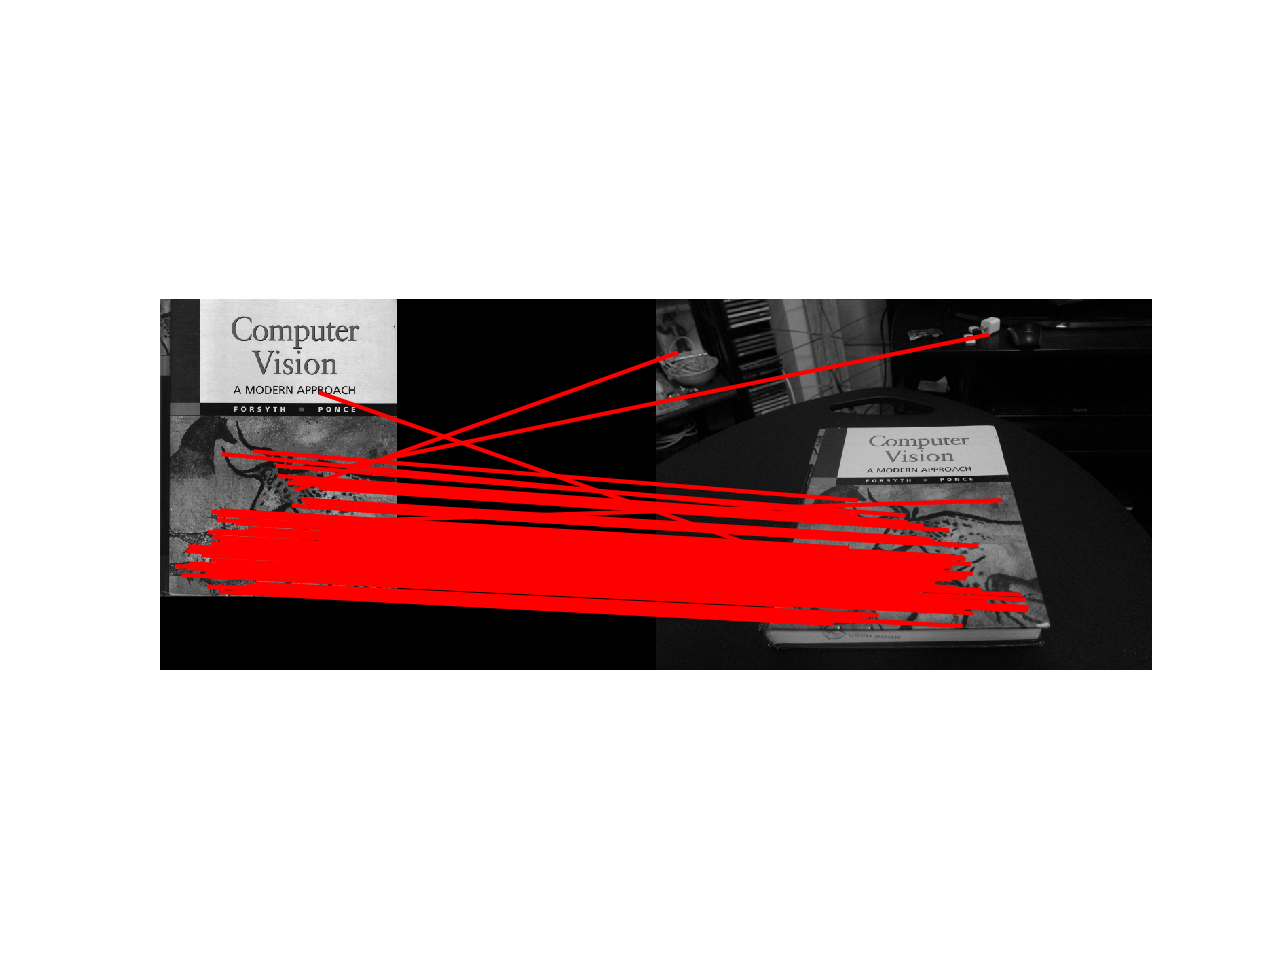
\includegraphics[width=0.4\textwidth]{results/q2_1_4_05_7.png}}
\subfigure[sigma=0.15 ratio=0.7]{
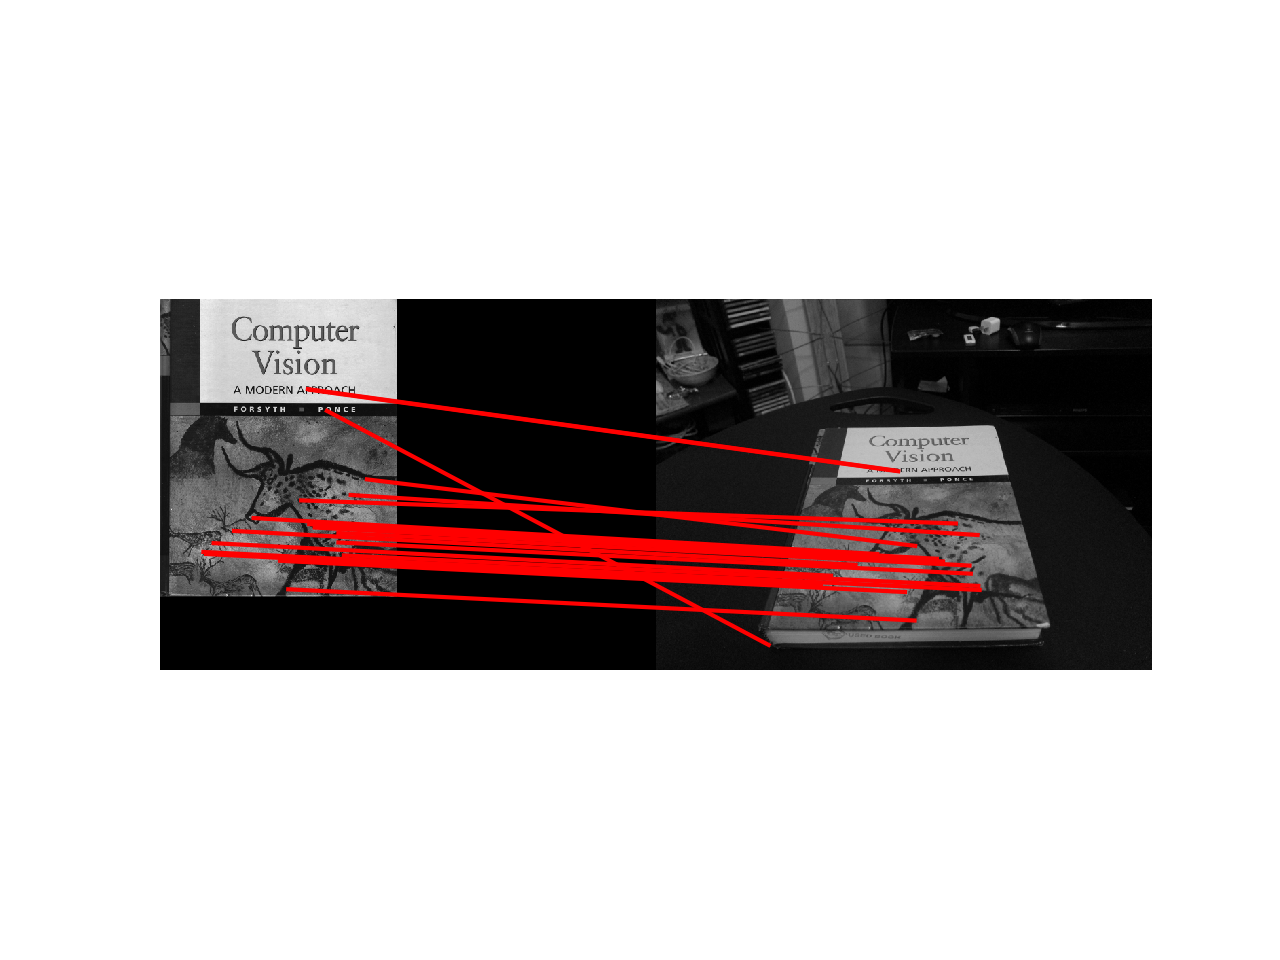
\includegraphics[width=0.4\textwidth]{results/q2_1_4_de.png}}
\subfigure[sigma=0.35 ratio=0.7]{
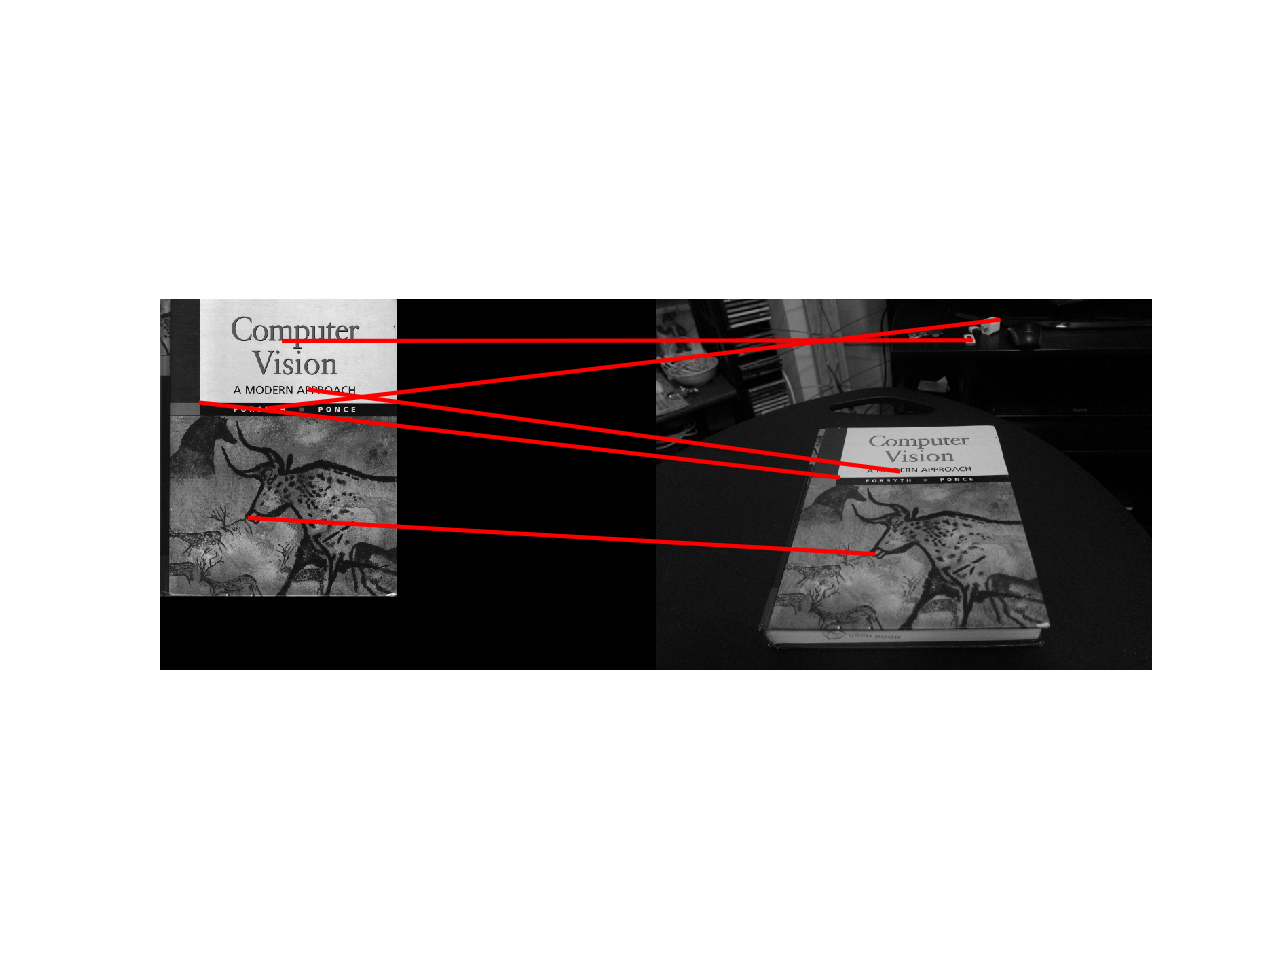
\includegraphics[width=0.4\textwidth]{results/q2_1_4_35_7.png}}
\subfigure[sigma=0.65 ratio=0.7]{
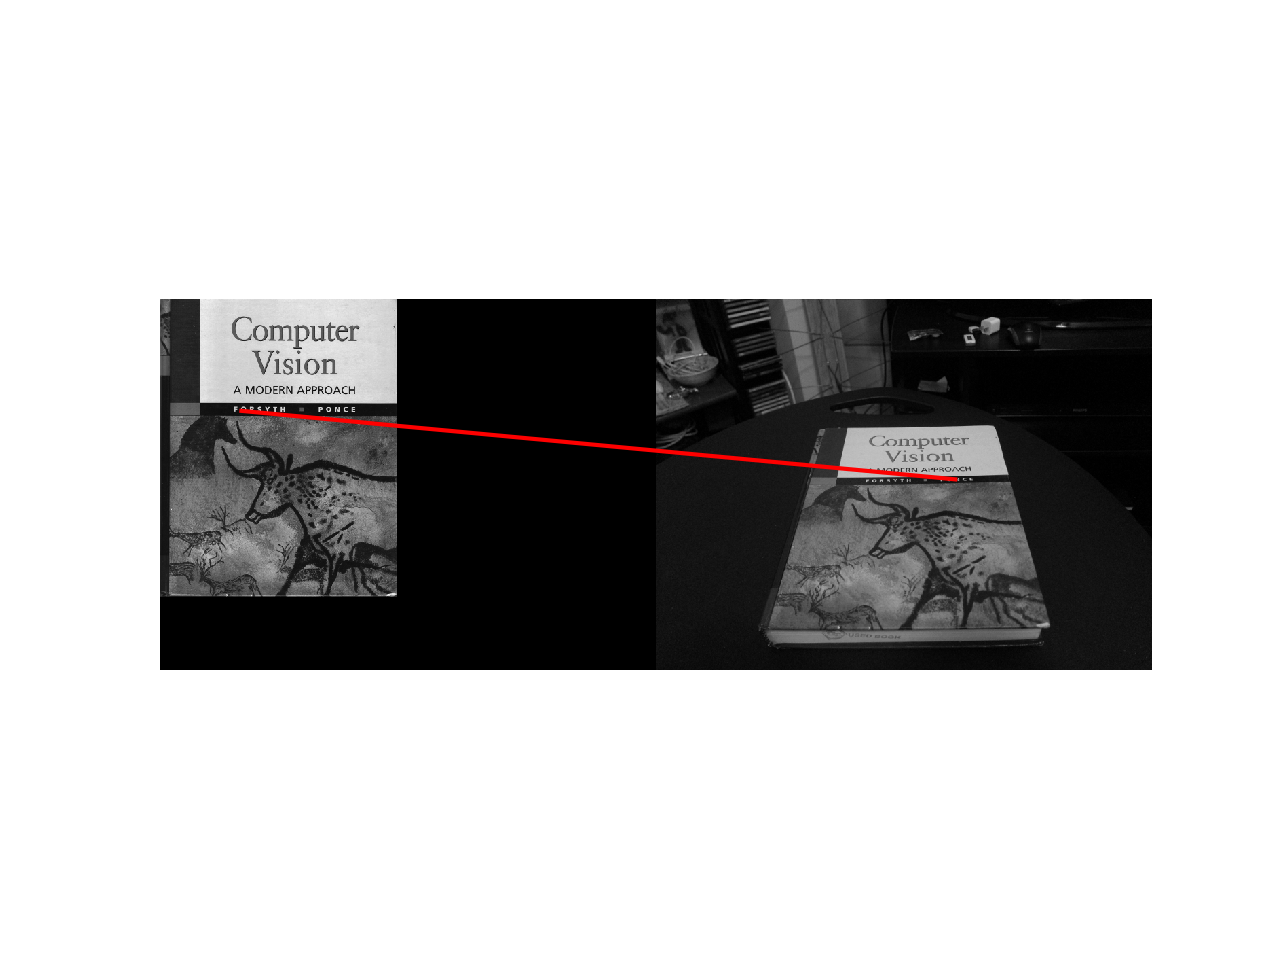
\includegraphics[width=0.4\textwidth]{results/q2_1_4_65_7.png}}
\end{figure}

As observed in the results. with the increase of ratio, matched points number increased drastically and when the ratio dropped, there would be fewer matched points, this is due to fewer point pairs would be considered matched with the drop of ratio. And increasing sigma would decrease matched points. That is, sigma is the threshold for corner detection and increase sigma would lead to less detected corner so that there would be fewer interest points for descriptor.

\subsubsection{BRIEF and Rotations}

In this case, with BRIEF feature descriptor ratio $ratio = 0.7$, I visualized match result for rotation angle $60, 180, 270$, images are shown below:
\begin{figure}[H]
\centering
\subfigure[rotate angle = 60]{
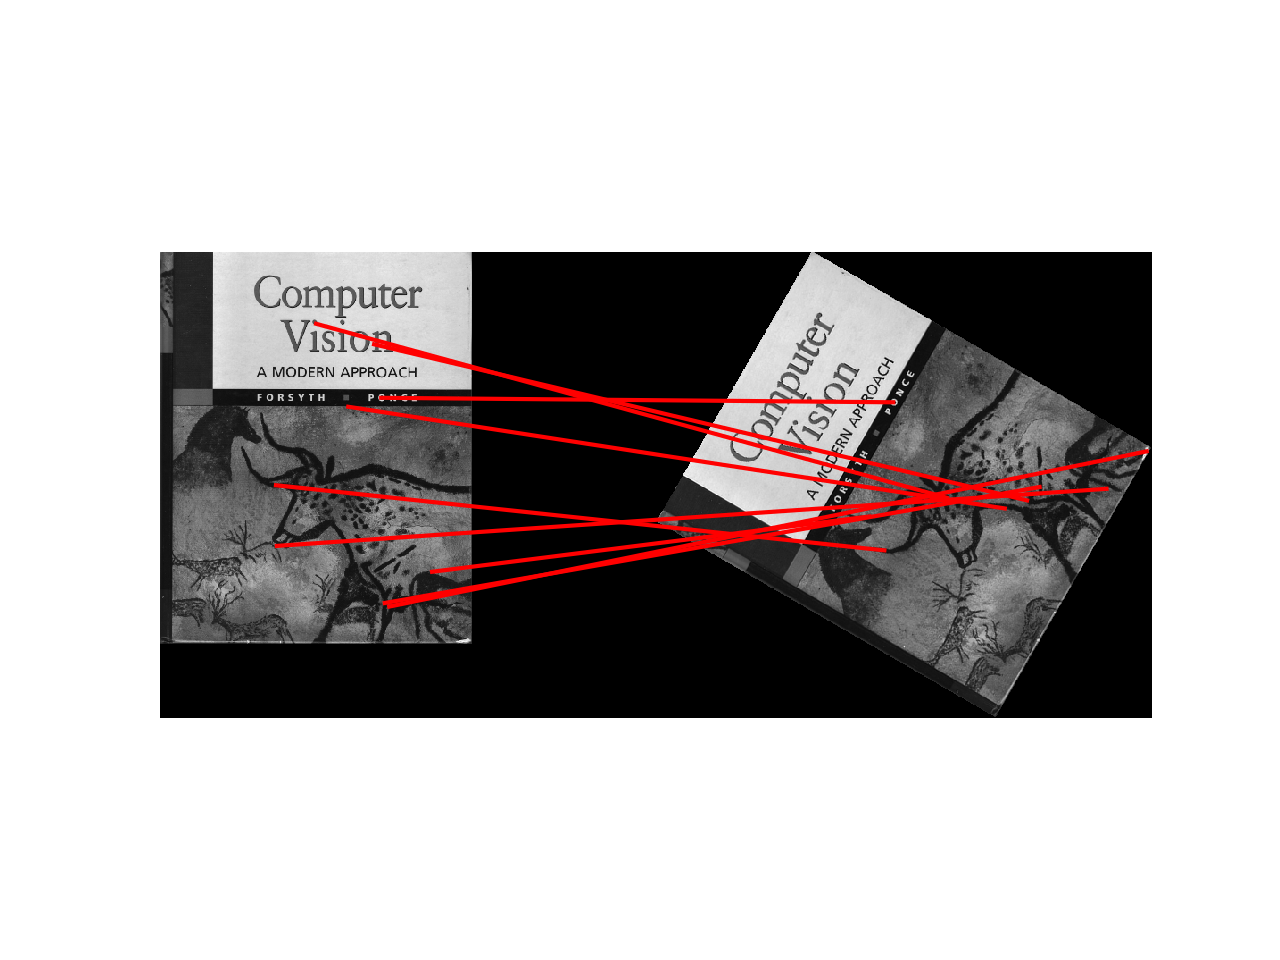
\includegraphics[width=0.3\textwidth]{results/q2_1_6_60.png}}
\subfigure[rotate angle = 180]{
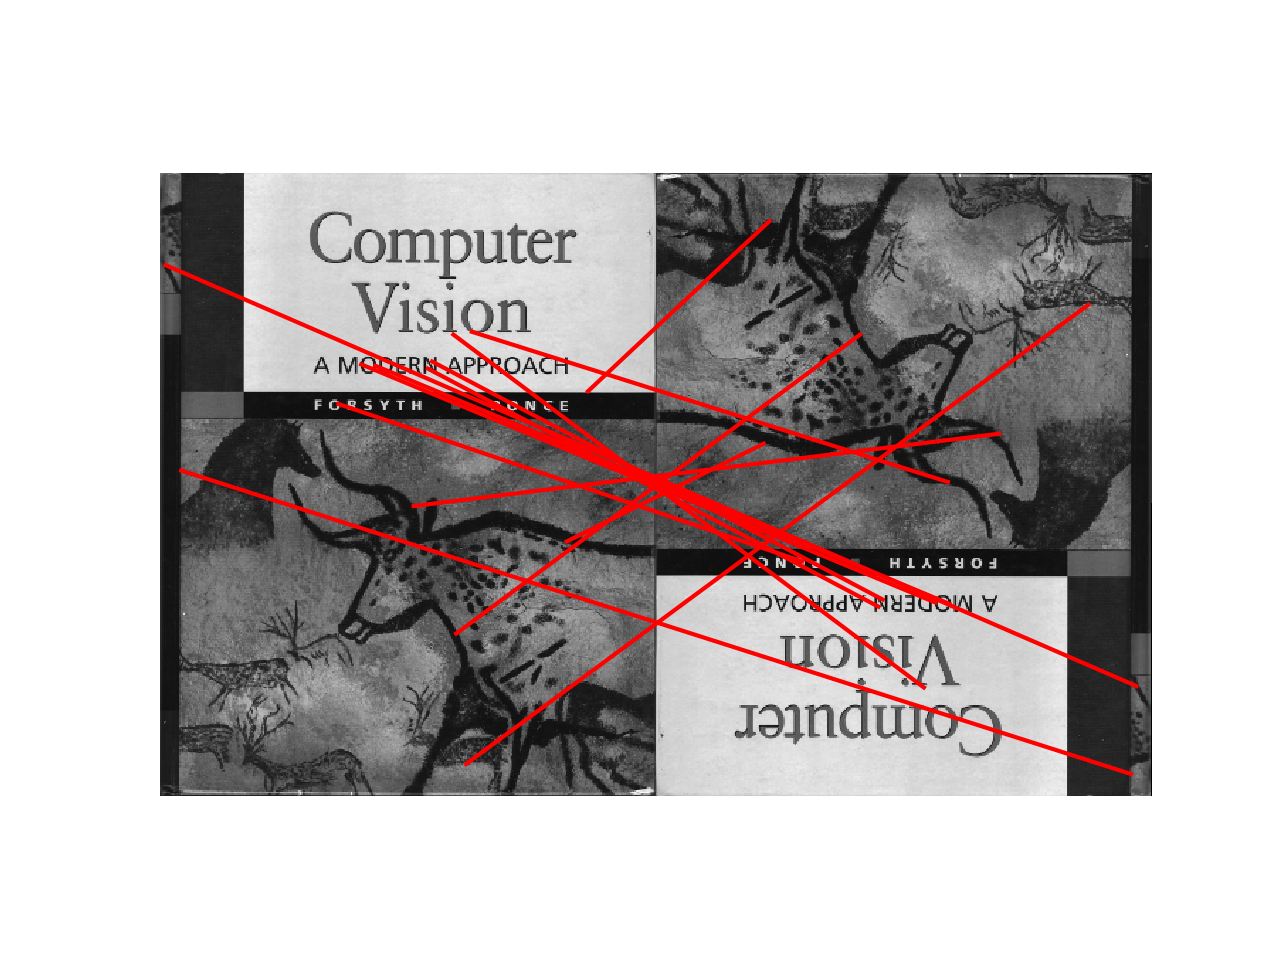
\includegraphics[width=0.3\textwidth]{results/q2_1_6_180.png}}
\subfigure[rotate angle = 270]{
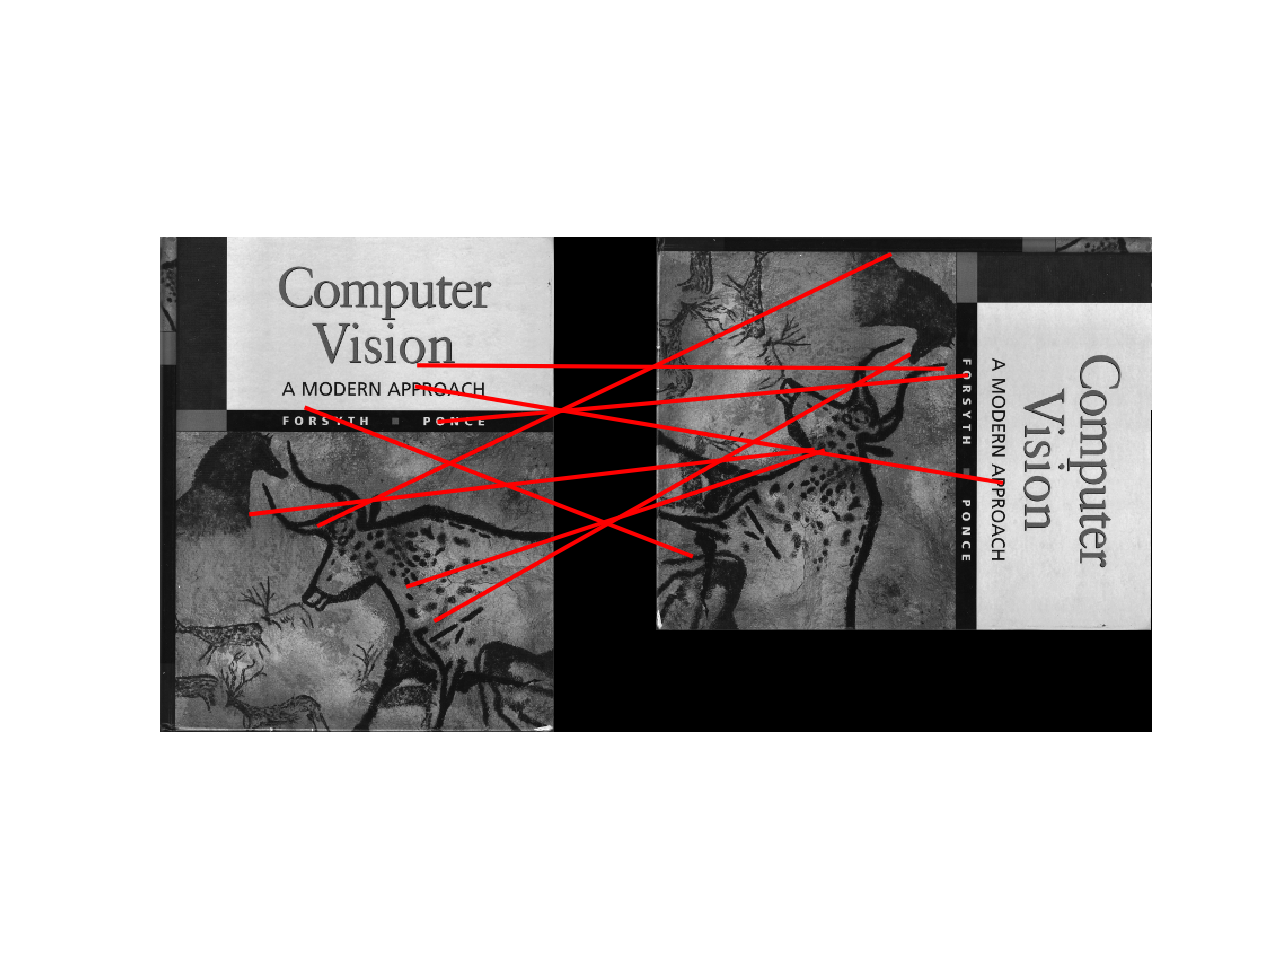
\includegraphics[width=0.3\textwidth]{results/q2_1_6_270.png}}
\end{figure}

The histogram is shown below:
\begin{figure}[H]
\centering
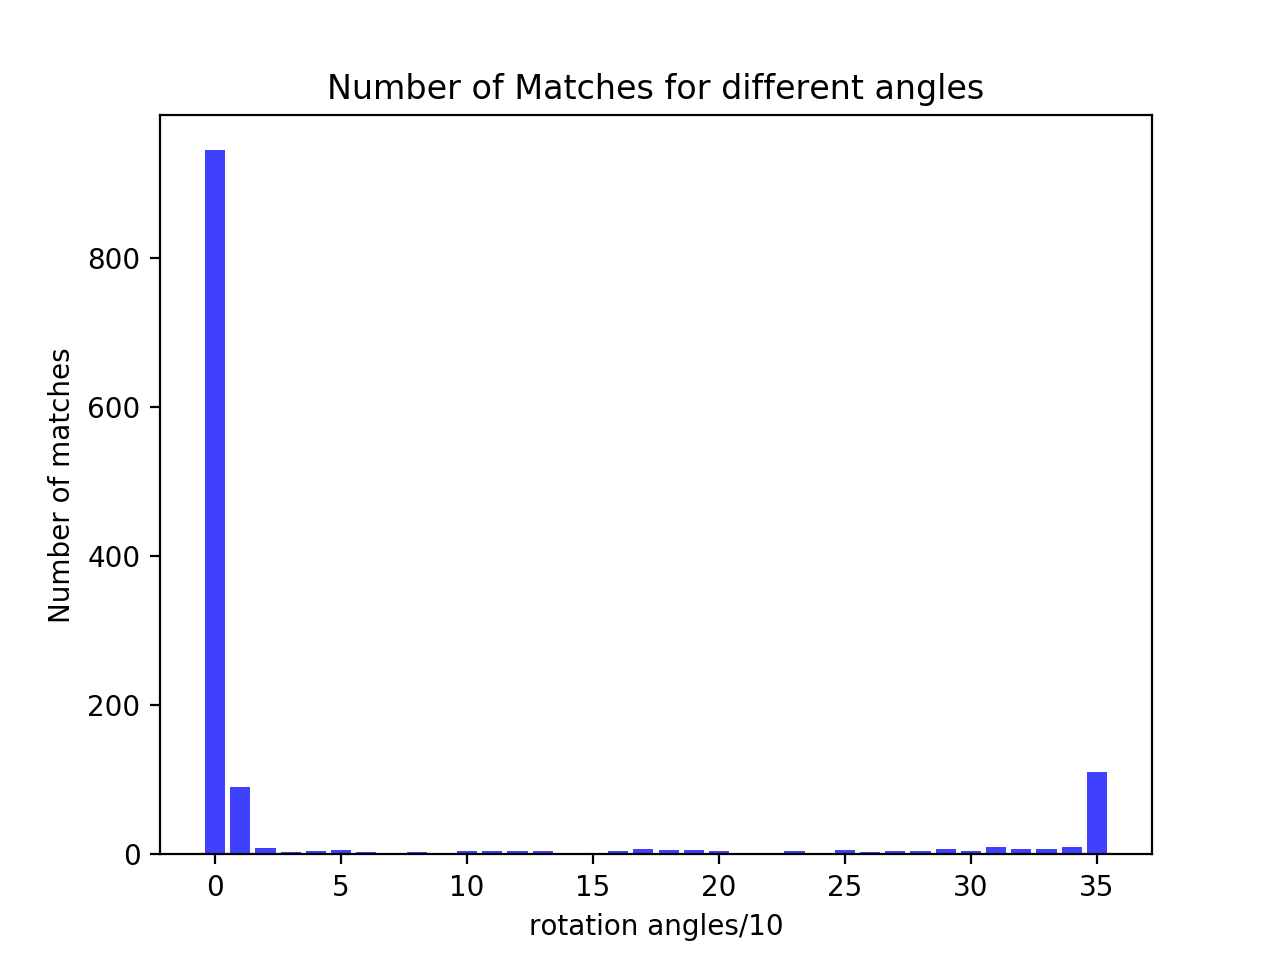
\includegraphics[width=0.5\textwidth]{results/q2_1_6_his.png}
\caption{resulting histogram}
\end{figure}

As was observed in results, the number of matches dropped drastically as the rotation angle increased. This is because BRIEF descriptors construct a bitset descriptor for each patch by comparing randomly chosen pixels location. When rotating the image, the keypoints are bound to give different descriptors for the same patch, and the comparison would occur at different pixel intensities.

\setcounter{subsection}{1}
\subsection{Homography Computation, Normalization and RANSAC}

\setcounter{subsubsection}{3}
\subsubsection{Putting it together}

Warped image is shown below:
\begin{figure}[H]
\centering
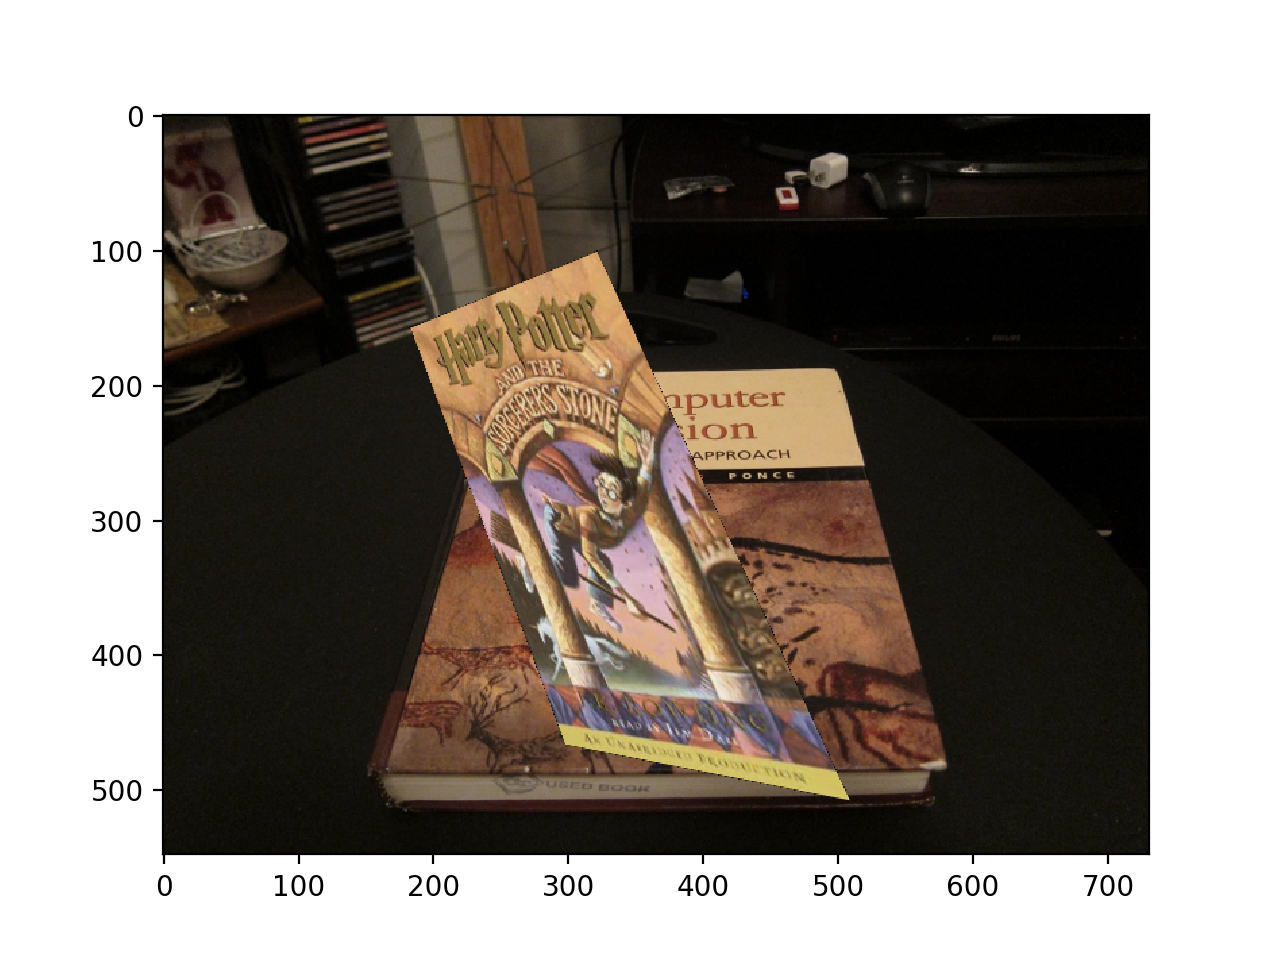
\includegraphics[width=0.5\textwidth]{results/q2_2_4.png}
\caption{warped image}
\end{figure}

Noticed that the hp\_cover image was placed in the right place but with a wrong size. The way to solve this problem could be increase iteration number to find a better homography, resize hp\_cover to a more precise shape, and decrease tolerance.

\subsubsection{RANSAC Parameter Tuning}

Since increase iteration number could increase the possibility to find optimized homography, so first I used default tolerance $2$ and changed numbers of iteration, the composited image became:
\begin{figure}[H]
\centering
\subfigure[iteration number=250, tolerance=2]{
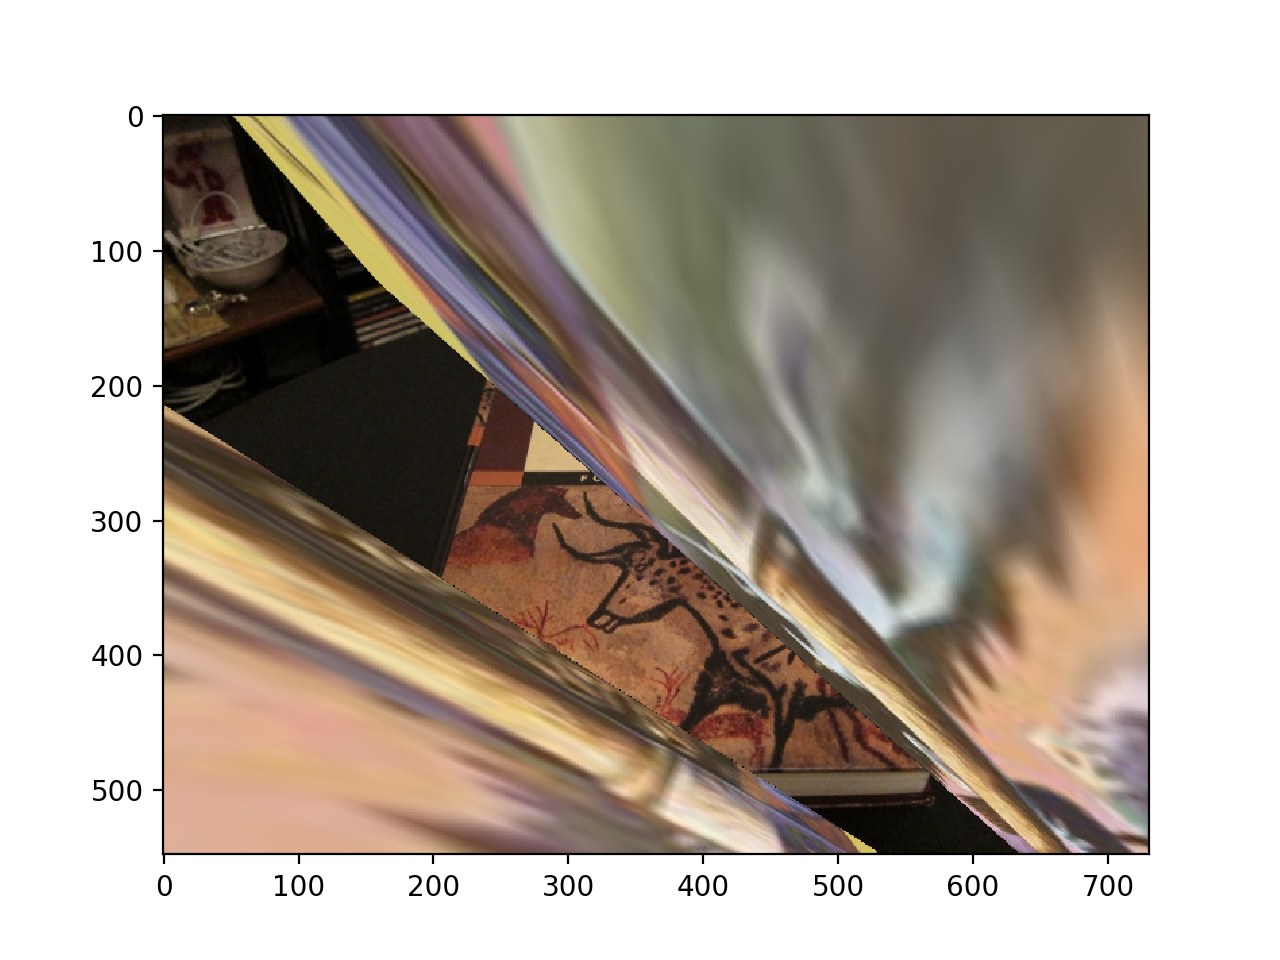
\includegraphics[width=0.4\textwidth]{results/q2_2_4_250_2.png}}
\subfigure[iteration number=750, tolerance=2]{
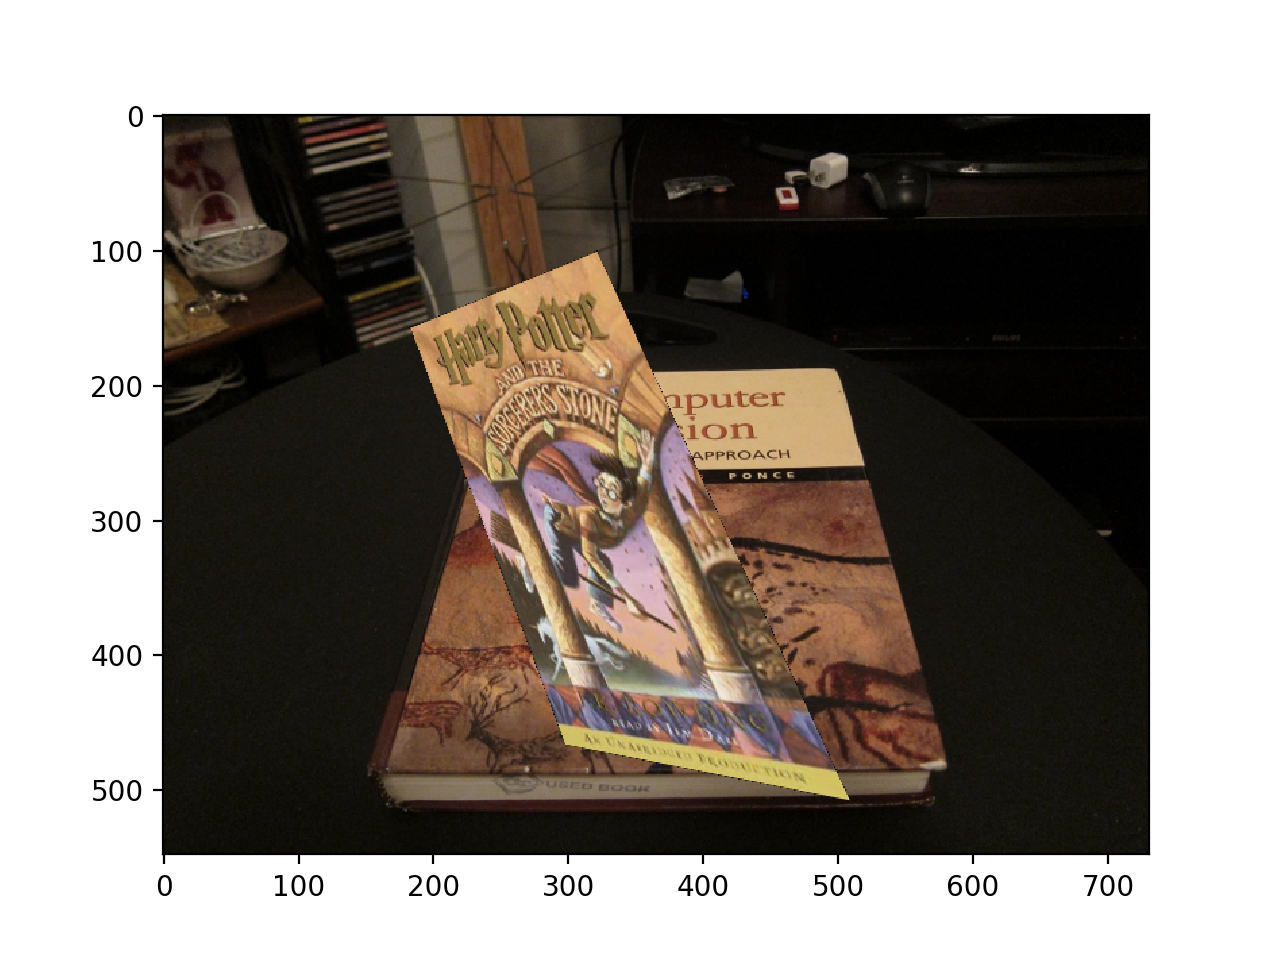
\includegraphics[width=0.4\textwidth]{results/q2_2_4_750_2.png}}
\subfigure[iteration number=1000, tolerance=2]{
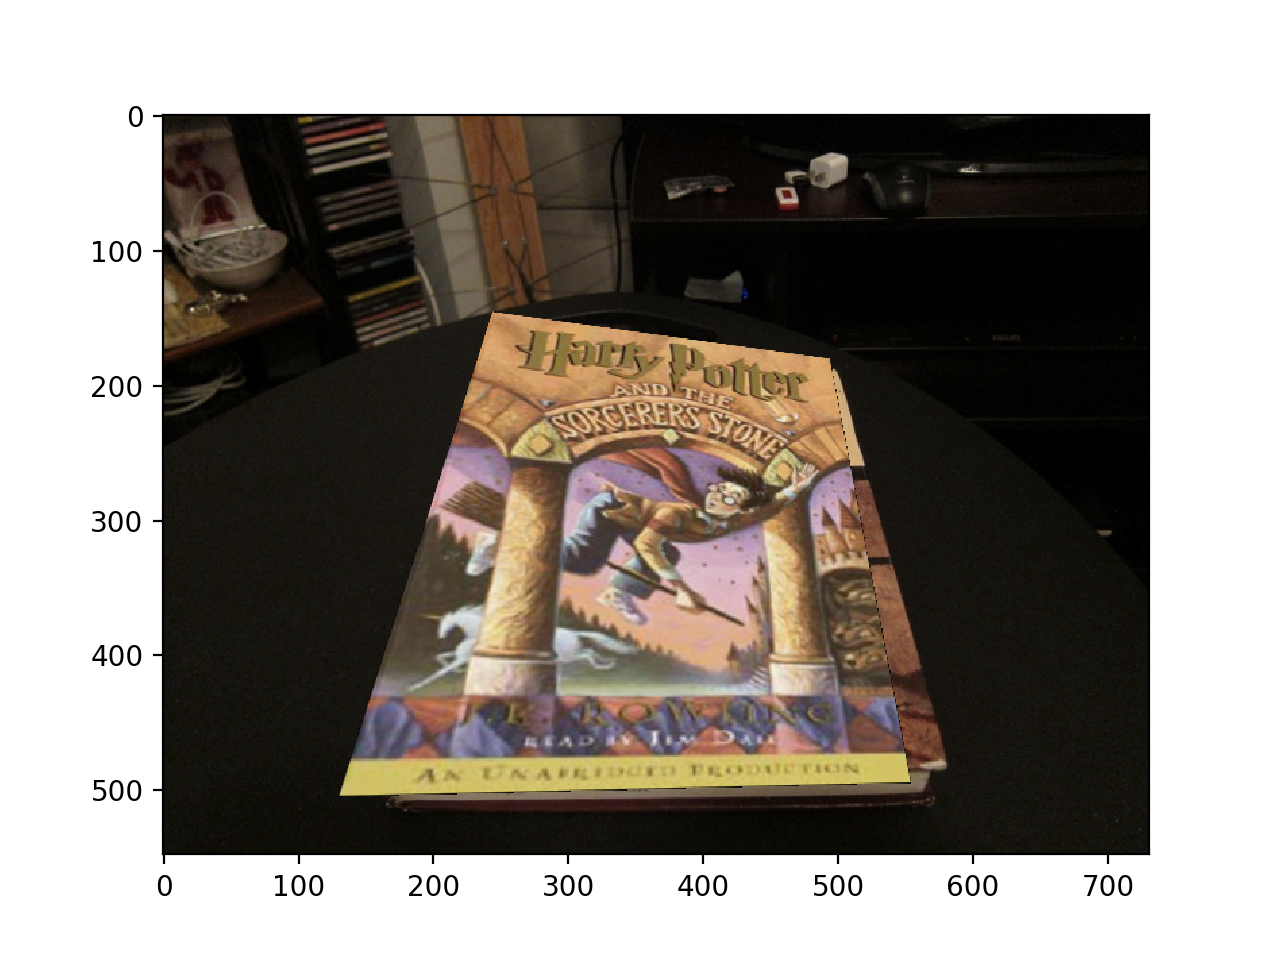
\includegraphics[width=0.4\textwidth]{results/q2_2_4_1500_2.png}}
\subfigure[iteration number=1500, tolerance=2]{
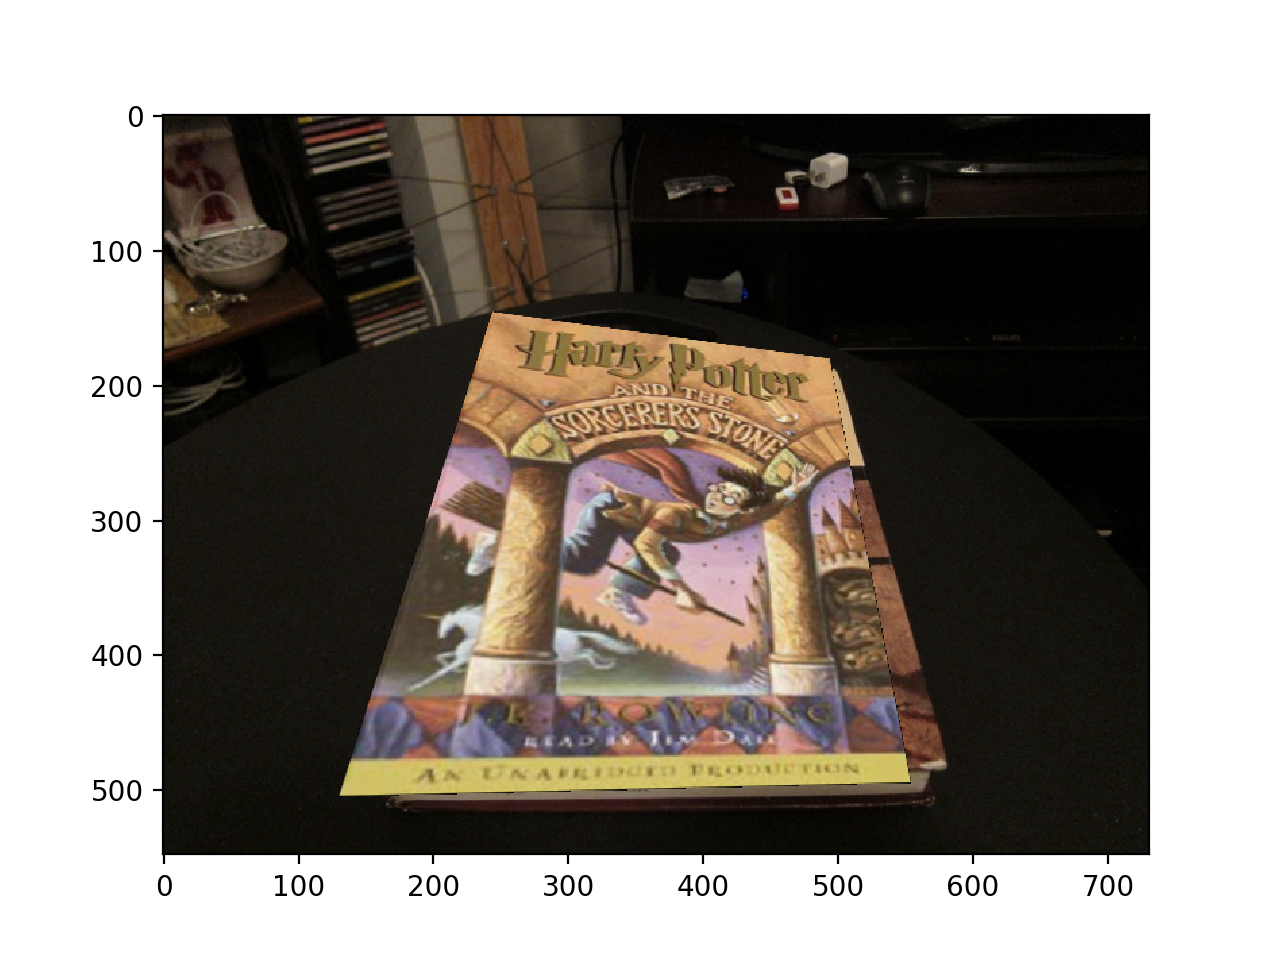
\includegraphics[width=0.4\textwidth]{results/q2_2_4_1500_2.png}}
\subfigure[iteration number=2000, tolerance=2]{
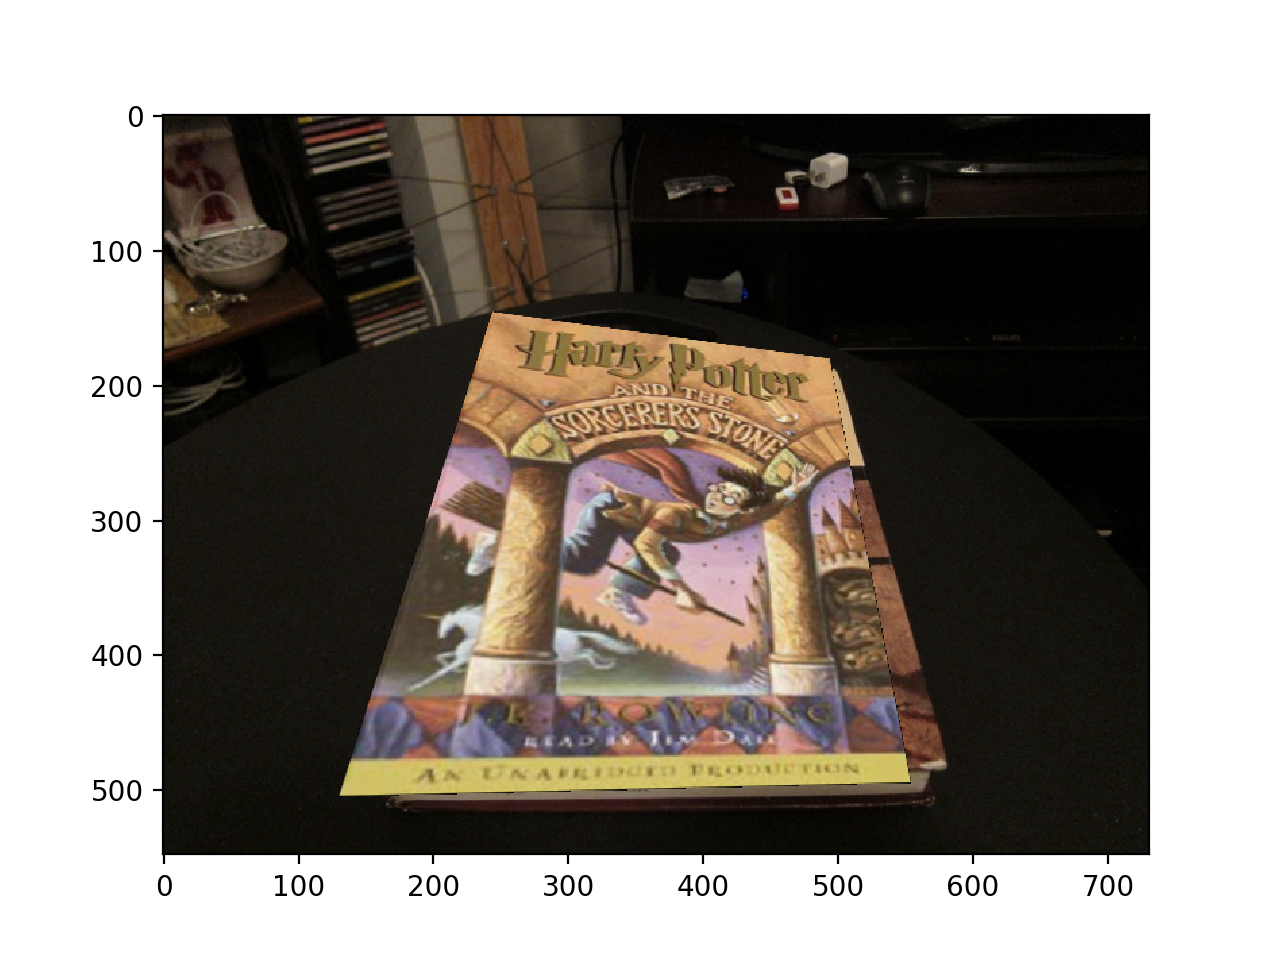
\includegraphics[width=0.4\textwidth]{results/q2_2_4_2000_2.png}}
\subfigure[iteration number=2500, tolerance=2]{
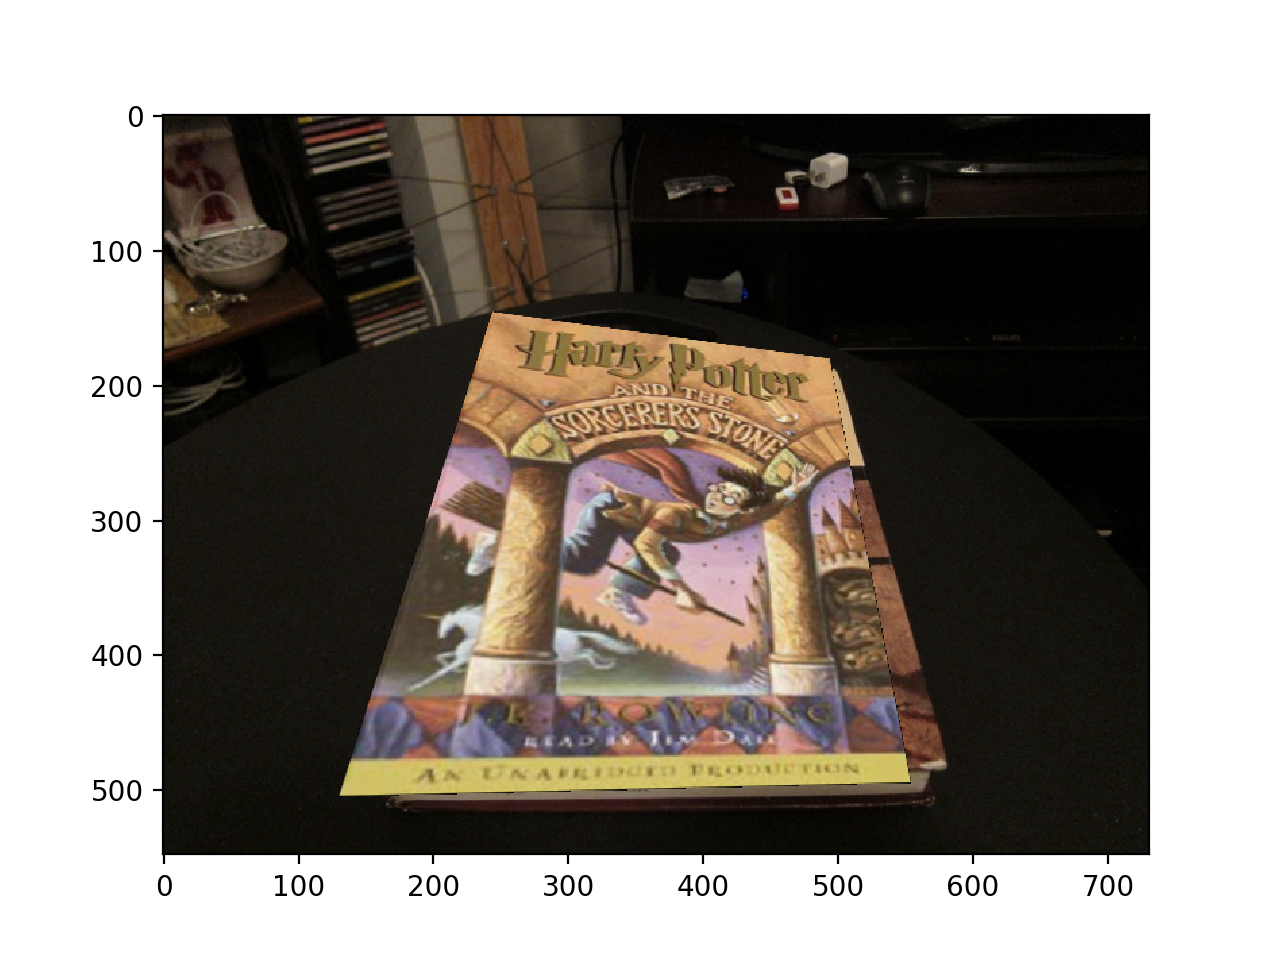
\includegraphics[width=0.4\textwidth]{results/q2_2_4_2500_2.png}}
\end{figure}

Noticed that as the iteration number increased, the warping image fitted slightly better because with more iteration we could acquire a better homography. So choose iteration number $1500$, the next step is to tune tolerance. Results are shown below:
\begin{figure}[H]
\centering
\subfigure[iteration number=1500, tolerance=1]{
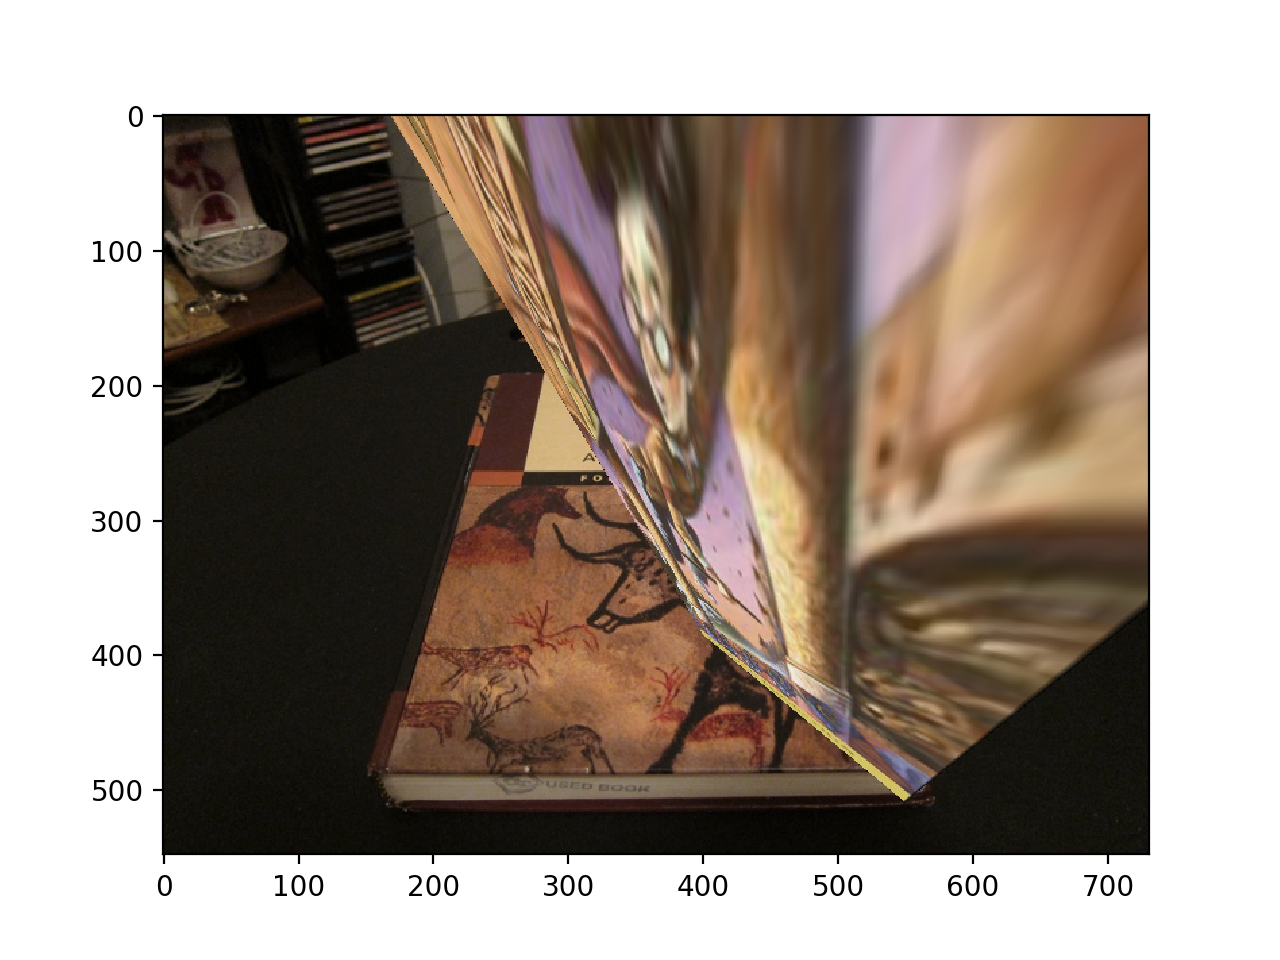
\includegraphics[width=0.4\textwidth]{results/q2_2_4_1000_1.png}}
\subfigure[iteration number=1500, tolerance=1.5]{
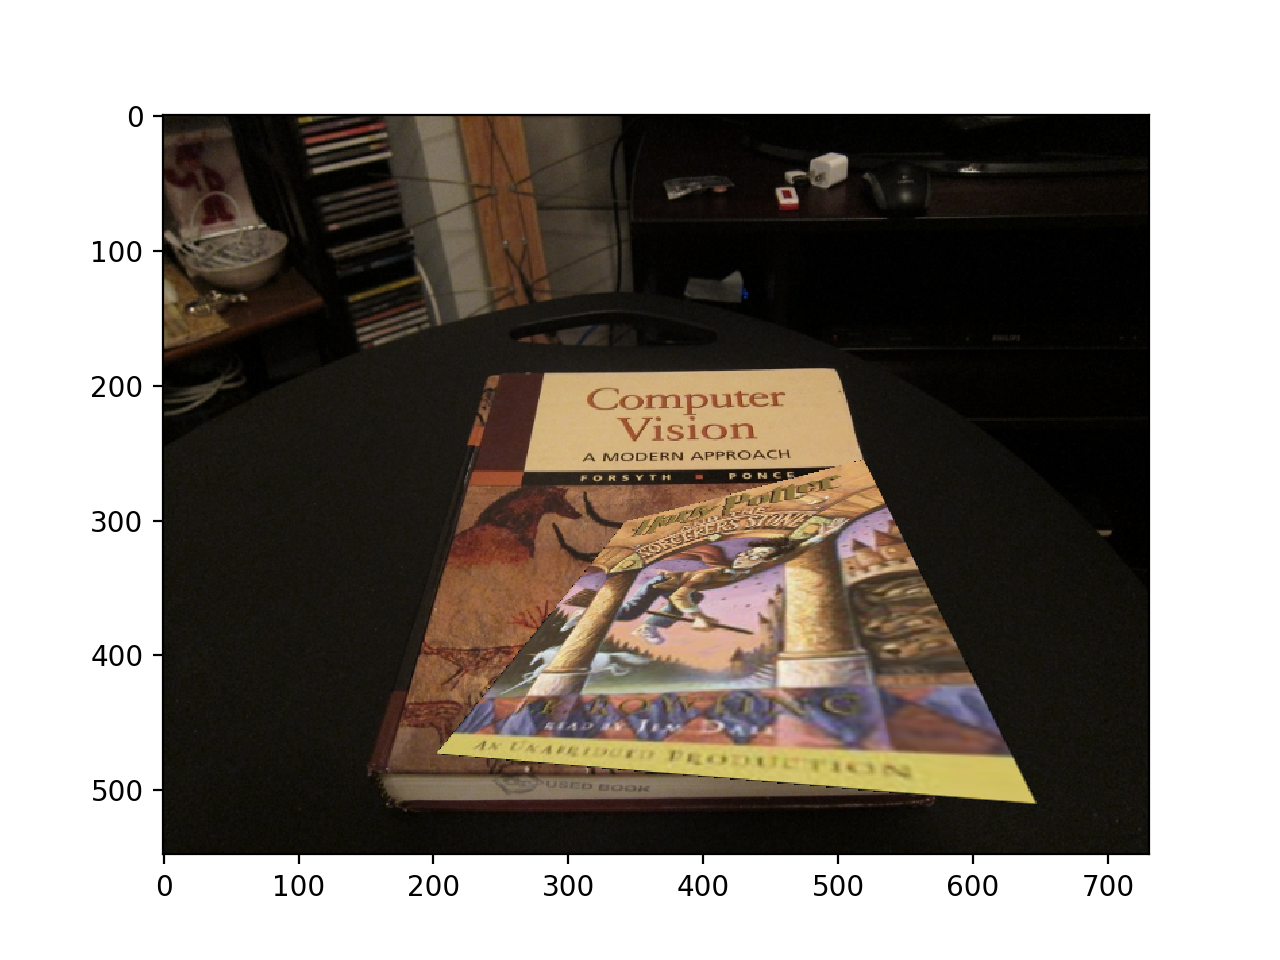
\includegraphics[width=0.4\textwidth]{results/q2_2_4_1000_15.png}}
\subfigure[iteration number=1500, tolerance=3]{
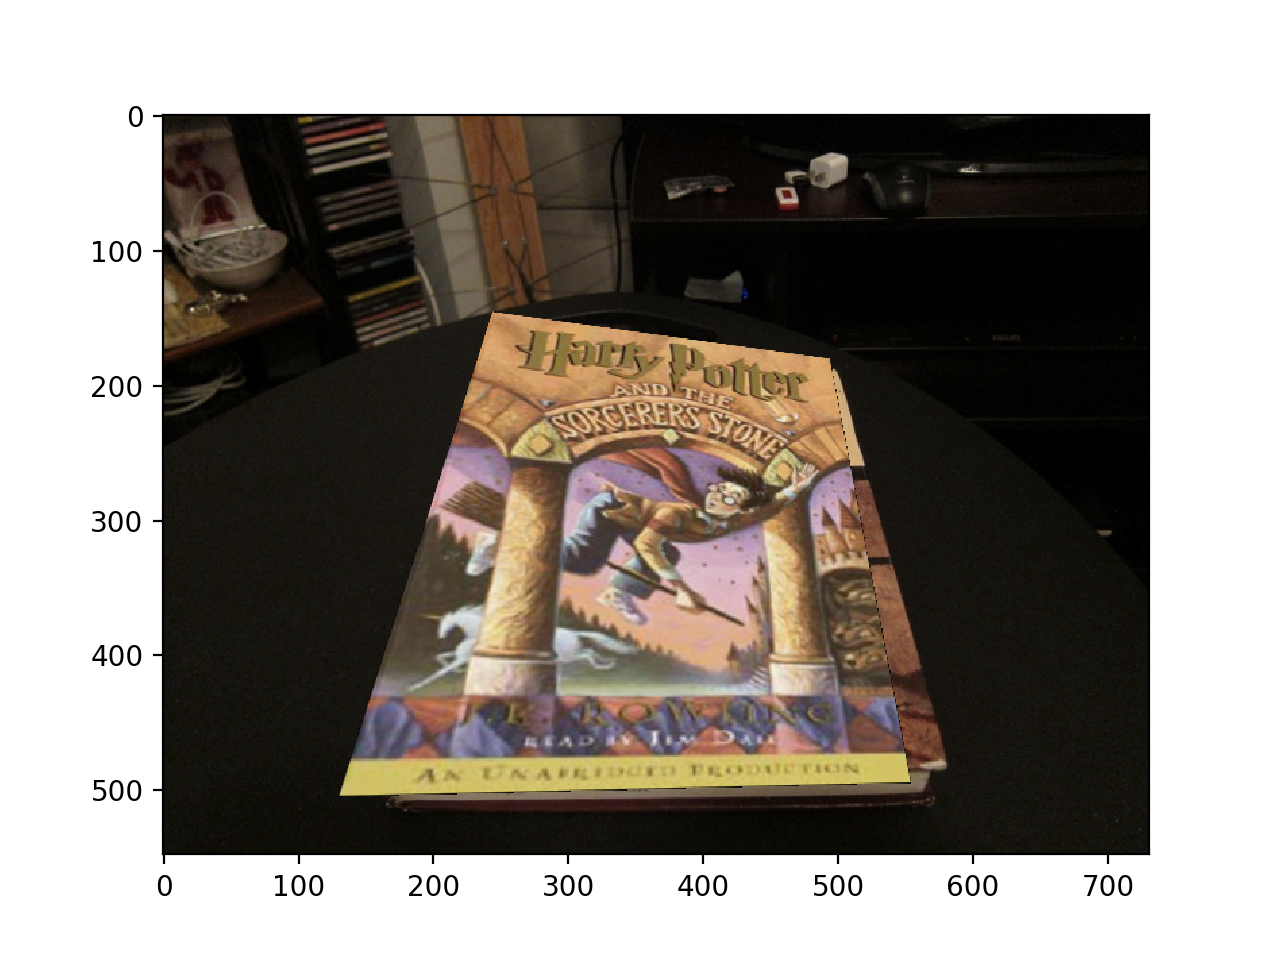
\includegraphics[width=0.4\textwidth]{results/q2_2_4_1000_3.png}}
\subfigure[iteration number=1500, tolerance=4]{
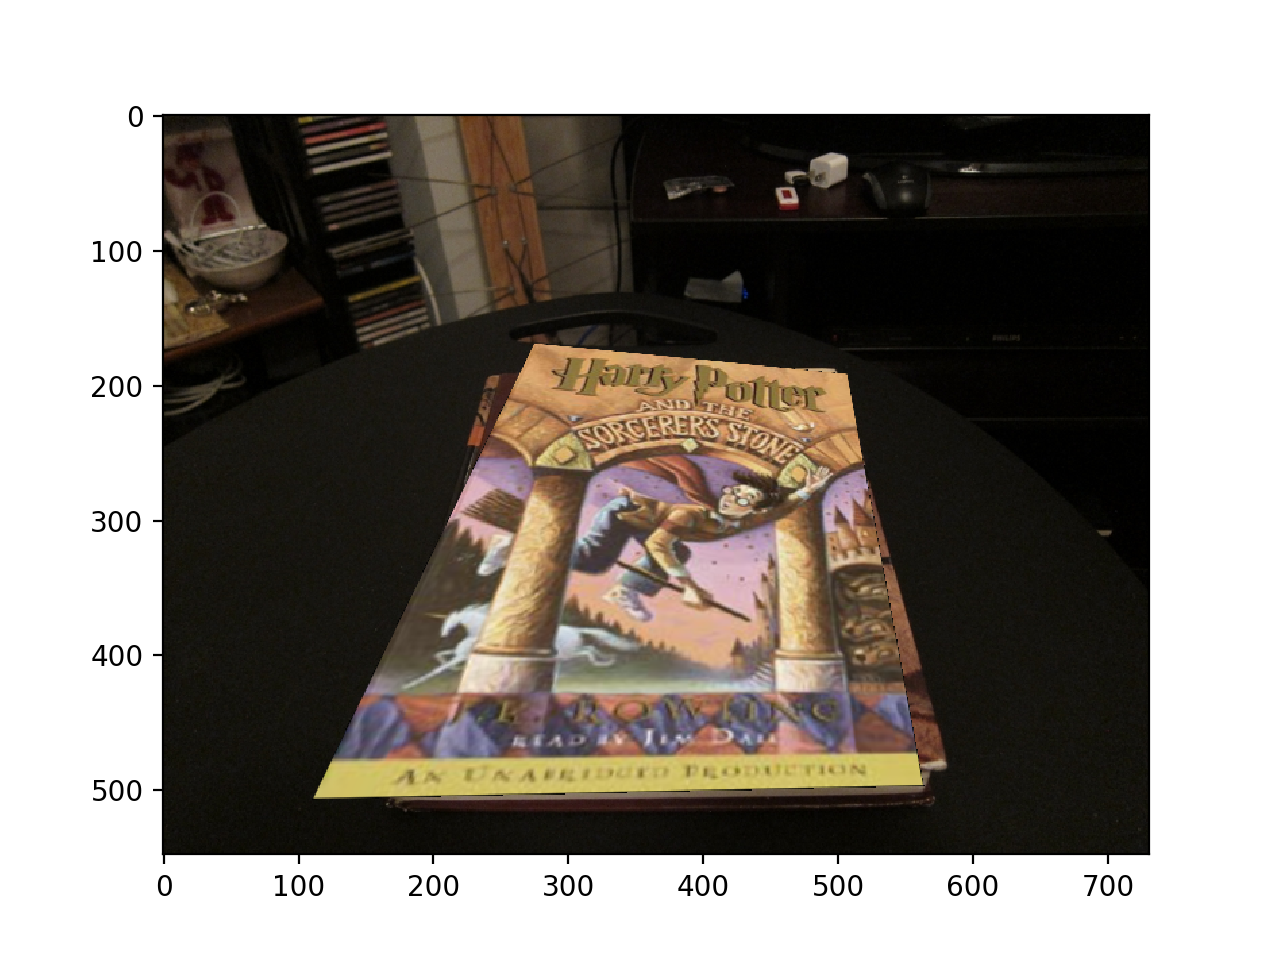
\includegraphics[width=0.4\textwidth]{results/q2_2_4_1000_4.png}}
\subfigure[iteration number=1500, tolerance=5]{
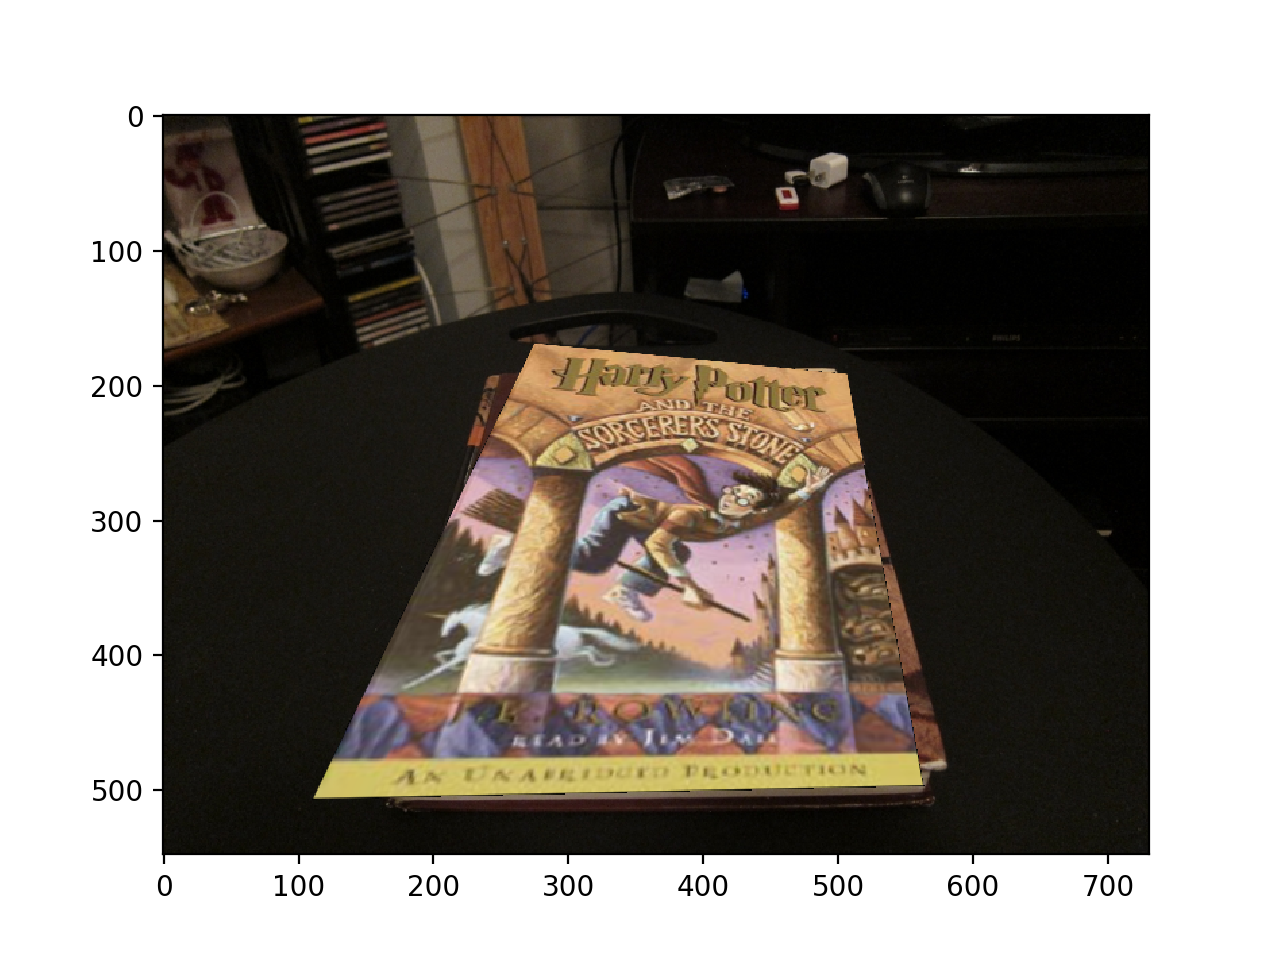
\includegraphics[width=0.4\textwidth]{results/q2_2_4_1000_5.png}}
\subfigure[iteration number=1500, tolerance=7]{
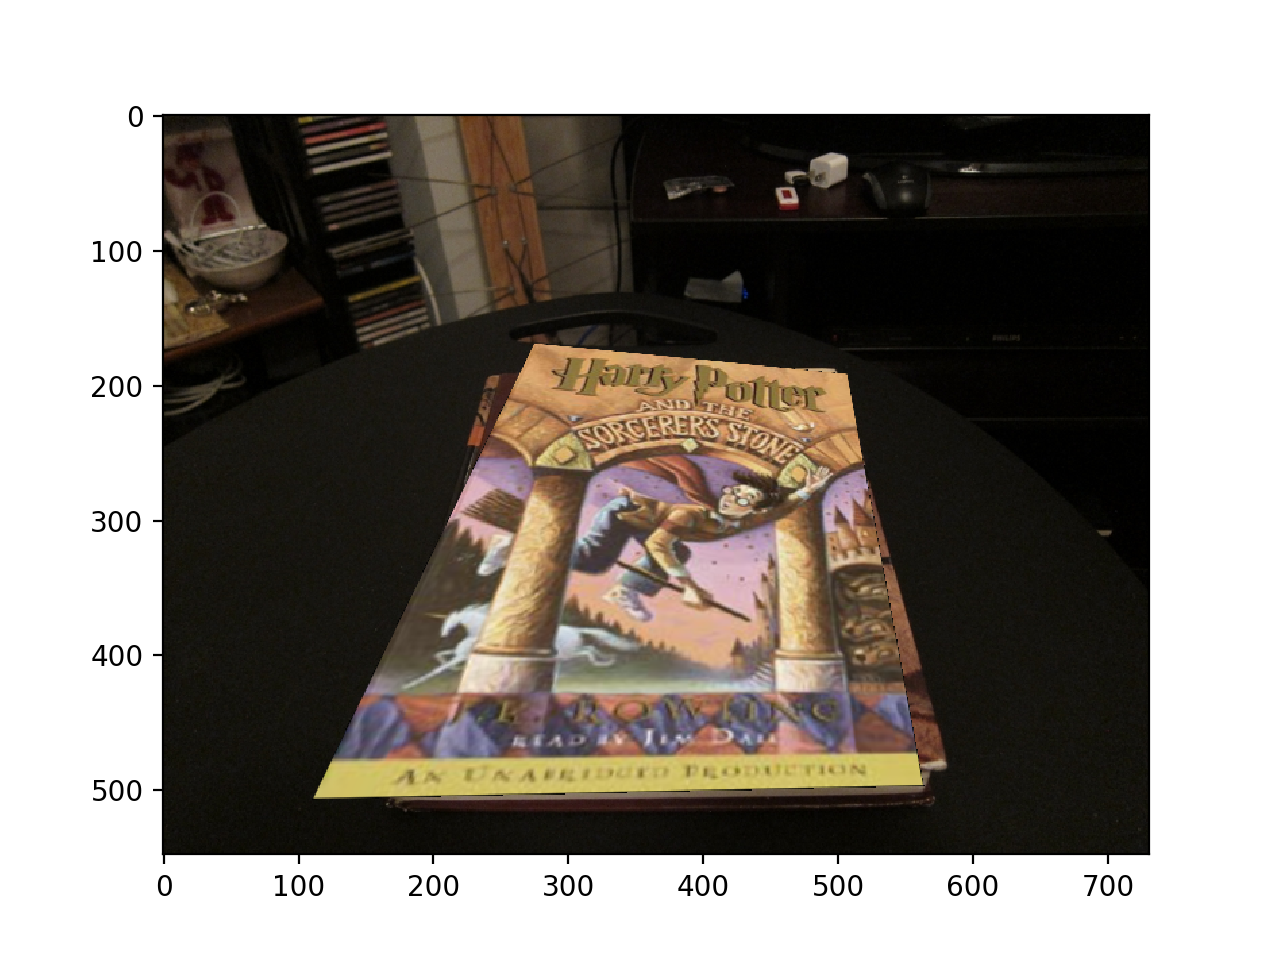
\includegraphics[width=0.4\textwidth]{results/q2_2_4_1000_7.png}}
\end{figure}

As observed in results, when tolerance increase, the template would have a better fit of image, since for tolerance larger than $3$ the results do not differ much, I would choose a tolerance as $3$.

\section{Creating your Augmented Reality Application}
\setcounter{subsection}{0}
\subsection{Incorporating Video}

\section{Extra Credit}
\setcounter{subsection}{1}
\subsection{Create a Simple Paranoma}

Created panaroma is shown below:
\begin{figure}[H]
\centering
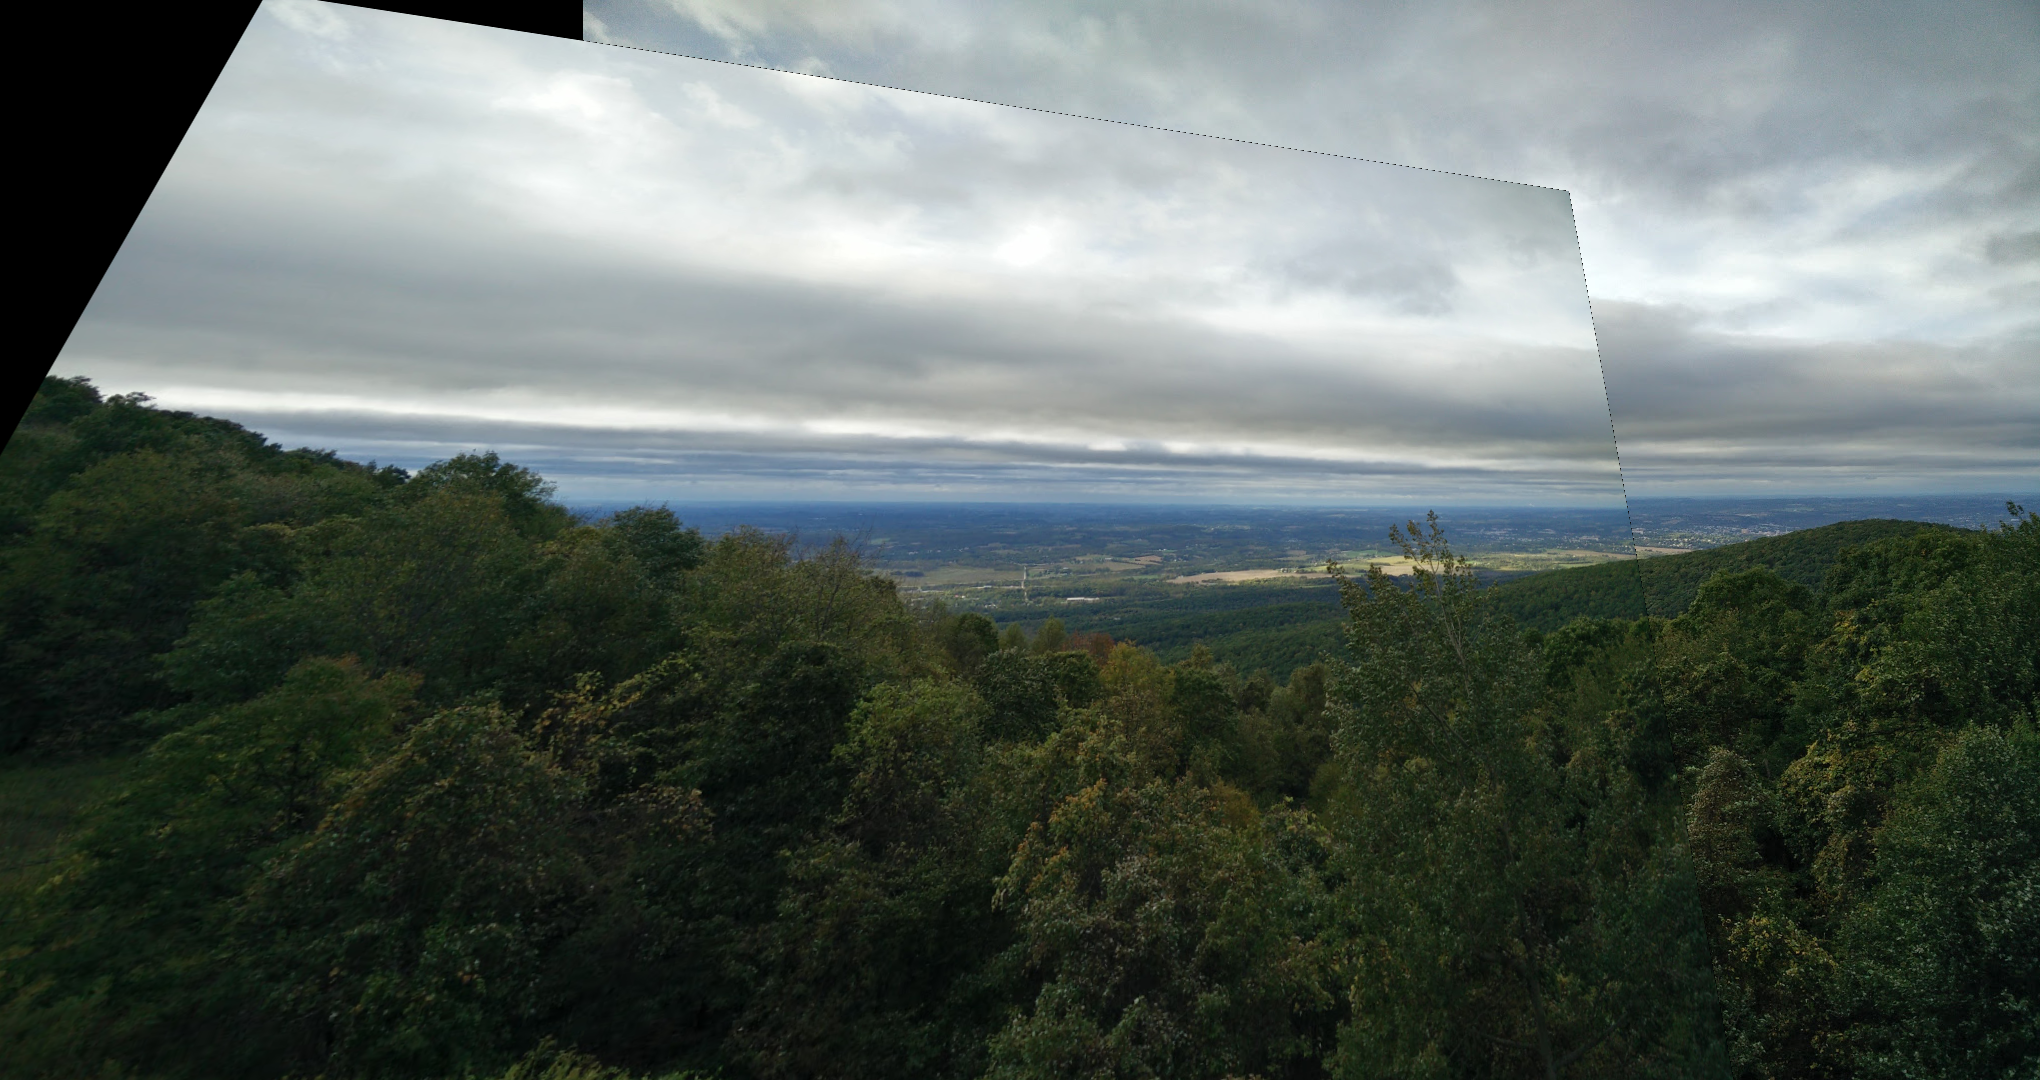
\includegraphics[width=0.5\textwidth]{results/pana.png}
\caption{paranoma}
\end{figure}

\end{document}
